\documentclass[type=doctor]{usststyle/usstthesis}
%type=[bachelor | master | doctor | postdoctor]
% 博士后论文:type=postdoctor
% 博士论文:type=doctor
% 硕士论文:type=masters
% 本科论文:type=bachelor
%本模版基于Tsinghua University Thesis Template(https://www.overleaf.com/latex/templates/tsinghua-university-thesis-template/wrjmnybpzbhw#.V_eZg-lh3Vo).

\usepackage{hyperref}%for \hypersetup
\usepackage{tikz}
% \hypersetup
% {
%     pdfauthor={Wangyan Li liwangyan618907@gmail.com},
%     pdftitle={The unofficial Latex thesis template for USST},
%     pdfkeywords={Latex, USST, Templatetikz}
% }

%\NewDocumentCommand \fangsong { } { \CJKfamily { zhsong } }

%\setCJKmainfont{simsun.ttc}%http://disq.us/t/1mrwb68 
 
%\setmainfont{Caladea} 
%\ctexset{fontset=ubuntu} 
% 选项:
%   type=[bachelor|master|doctor|postdoctor], % 必选
%   secret,                                   % 可选
%   pifootnote,                               % 可选(建议打开)
%   openany|openright,                     
 
% 所有其它可能用到的包都统一放到这里了,可以根据自己的实际添加或者删除。
\usepackage{usststyle/usstthesis}
\usepackage[flushleft]{threeparttable}
\usepackage{makecell,booktabs}  
\usepackage{tikz}
\usepackage{hyperref}
\usepackage{xeCJK}
\usepackage{ctex}
%\usepackage{cite}
%\usepackage{CJKutf8}
\usepackage{siunitx}
\usepackage{bm}
\usepackage{amsmath}
\usepackage{bbding}
\usepackage{amssymb}
\usepackage{pifont}

%\usetikzlibrary{arrows}
\usetikzlibrary{arrows.meta}
%\usepackage[ruled]{algorithm2e}
\usepackage{algorithm}
\floatname{algorithm}{\heiti 算法}
\usepackage{algpseudocode} % 必须包含此包以支持 \State

\renewcommand{\thealgorithm}{\thechapter.\arabic{algorithm}}
%\usepackage{mathptmx}
\usepackage{newtxmath}
\usepackage{changepage}

% \usepackage[style=thuthesis]{biblatex} % 样式通常在加载宏包时指定

% 定义所有的图片文件在 figures 子目录下
\graphicspath{{figures/}}

% 可以在这里修改配置文件中的定义。导言区可以使用中文。

%% MUST be in preamble for biblatex
%% And biblatex/biber can only take one file at a time. And needs the .bib extension.
% \bibliography{ref/full,ref/article,ref/conf,ref/me,ref/arXiv,ref/books} 
%\addbibresource{ref/full.bib}
%\addbibresource{ref/article.bib}
\addbibresource{ref/refs.bib}

%\addbibresource{ref/conf.bib}
\addbibresource{ref/chapter1.bib}
\addbibresource{ref/chapter2.bib}
\addbibresource{ref/chapter3.bib}
\addbibresource{ref/chapter4.bib}
%\addbibresource{ref/arXiv.bib}
%\addbibresource{ref/books.bib}




% \DeclareCiteCommand{\supercite}[\mkbibsuperscript]
%   {\iffieldundef{prenote}
%      {}
%      {\BibliographyWarning{Ignoring prenote argument}}%
%    \iffieldundef{postnote}
%      {}
%      {\BibliographyWarning{Ignoring postnote argument}}}
%   {\usebibmacro{citeindex}%
%    \bibopenbracket\usebibmacro{cite}\bibclosebracket}
%   {\supercitedelim}
%   {}
  
  % \let\cite=\supercite

\newcommand{\diag}{{\rm diag}}
\newcommand{\rank}{{\rm rank}}
\newcommand{\tr}{{\rm tr}}
\newcommand{\sign}{{\rm sign}}
\newcommand{\sgn}{{\rm sgn}}
\newcommand{\Proj}{{\rm Proj}}
\newcommand{\e}{{\rm e}}
\newcommand{\re}{{\rm Re}}
\begin{document}
\title{USST PHD THESIS}

% 封面部分
\includepdf[pages=-]{chapters/fengmian_zyd.pdf}
\frontmatter
\renewcommand{\thepage}{}
\begin{cabstract}


\end{cabstract}
\addtocontents{toc}{{\protect\noindent\protect\xiaosi 中文摘要\protect\par}}  %% 目的是在目录中出现中文摘要
% 如果习惯关键字跟在摘要文字后面,可以用直接命令来设置,如下:
\ckeywords{双足机器人 \quad 控制策略}

\hyphenpenalty=5000
\exhyphenpenalty=5000
\begin{eabstract}
\end{eabstract}
\addtocontents{toc}{{\protect\noindent\protect \textrm{ABSTRACT}\protect\par}}
\ekeywords{\textbf{Bipedal robot, Control Strategy}}
% % 如果使用授权说明扫描页,将可选参数中指定为扫描得到的 PDF 文件名,例如:
% % \makecover[scan-auth.pdf]
\makecover
% \includepdf[pages=-]{chapters/abstract_ch.pdf}
% \includepdf[pages=-]{chapters/abstract_en.pdf}
% \thispagestyle{empty}
% \addtocontents{toc}{{\protect\noindent\protect\heiti 中文摘要\protect\par}}  %% 目的是在目录中出现中文摘要
% \addtocontents{toc}{{\protect\noindent\protect\bfseries ABSTRACT\protect\par}}

%% 目录
\tableofcontents 

%% 符号对照表


%%% 正文部分
\mainmatter
%    \chapter{绪论}
\section{研究背景与意义}
% 基于任务优先级的人形机器人腿臂协同控制研究
近年来,人工智能技术在感知、认知与决策层面取得了突破性进展。现有系统已经能够在复杂场景中实现高精度的目标识别\cite{russakovsky2015imagenet},合成高分辨率、逼真的照片级图像\cite{brock2018large,karras2019style},根据自然语言描述自动生成具有实用价值的程序代码\cite{brown2020language,chen2021evaluating},并在多种具有挑战性的游戏环境中超越人类顶尖水平\cite{berner2019dota,arulkumaran2019alphastar,silver2016mastering}。然而,与其在感知与认知能力上的快速发展相比,人工智能体在物理世界中的运动能力仍显著落后于人类及其他生物所展现出的灵活性与适应性。

人类之所以能够在复杂、动态且高度不确定的环境中完成多样而精细的运动行为,得益于人类长期进化形成的高度协调的全身运动控制机制,尤其体现在上下肢之间的协同配合与任务分工上。相比之下,当前的机器人系统,无论是在仿真环境还是现实部署中,往往只能执行少量预定义或高度专用的动作,其行为形式僵化、鲁棒性有限,难以应对真实环境中的复杂扰动和突发状况。这种差距在双足人形机器人上尤为突出。

具备类人运动能力的双足人形机器人,被普遍认为是未来服务机器人、特种机器人以及人机协作系统的重要发展方向。若能够显著提升其全身运动控制能力,使其在非结构化环境中稳定完成诸如坐下、起立、跌倒与爬起等高风险、高自由度动作,将有助于机器人从实验室和受控工业场景中走向更加真实、复杂的应用环境。同时,具有自然、协调运动模式的虚拟人和机器人智能体,也将在计算机图形学、虚拟现实、生物力学以及康复医学等领域展现重要价值。

围绕上述目标,研究者提出了多种控制器设计方法。传统的基于模型的手工设计控制策略在复现人类敏捷性方面已取得一定成果\cite{raibert2012hopping,mcgeer1990passive,raibert1991animation,schwind1998spring,geyer2003positive,vukobratovic2004zero,yin2007simbicon,da2008simulation,bledt2018cheetah,}。然而,尽管人类能够熟练完成各类全身运动技能,其内在控制机理却难以被清晰刻画,更难以将其系统性地编码进控制器之中。

在机器人领域,手工设计控制器同样取得了一些令人信服的成果 \cite{raibert1984experiments,miura1984dynamic,hodgins1995animating,coros2010generalized,hutter2016anymal}。但此类方法通常高度依赖专家经验与大量精细调参,所得到的控制器往往针对特定任务或技能进行定制,难以自然扩展到更大规模、更丰富的技能集合。当研究对象转向难度更高、专业性更强的行为(如坐起或爬起)时,由于接触关系更加复杂、系统动力学更难精确建模,控制器的设计与调试过程将显著复杂化。总体而言,尽管手工设计方法取得了诸多成功,其所能达到的运动表现仍与人类所展现出的丰富性、灵活性与优雅性存在明显差距。

为降低控制器设计的人工成本,基于优化的方法,如模型预测控制(MPC)\cite{de2010feature,sreenath2011compliant,mordatch2012discovery,al2012trajectory,gehring2016practice,dogar2011framework,apgar2018fast} 与强化学习(RL)\cite{van1994virtual,kohl2004policy,tedrake2004stochastic,endo2005learning,coros2009robust,tan2018sim,haarnoja2018learning,hwangbo2019learning},逐渐成为合成复杂运动技能的重要工具。这类方法通过优化目标函数来自动搜索控制策略,将设计者的主要工作从“如何控制”转变为“希望智能体表现出何种行为”。其中,强化学习在合成高自由度、强非线性系统的运动控制策略方面表现出强大潜力,已被成功应用于多种仿人运动技能的学习 \cite{wang2012optimizing,tan2014learning,levine2016end,peng2016terrain,gu2017deep,andrychowicz2020learning}。

然而,基于优化的方法在实际应用中仍面临显著挑战。目标函数的设计往往需要融合大量领域知识,并对任务高度敏感。例如,仅为了诱导智能体产生自然的人类步态,就需要在能量效率、对称性、冲击力抑制以及稳定性等多个维度之间进行精细权衡\cite{wang2009optimizing,mordatch2012discovery,geijtenbeek2013flexible,clegg2018learning,yulearning,abdolhosseini2019learning}。当任务扩展至坐下起立、跌倒爬起等更具挑战性的动作时,这种基于目标函数的设计方式不仅调参成本高,而且难以系统性地刻画人类动作中隐含的腿部与上肢的协同控制规律。这不禁引人思考:是否有一种方法能够根据任务来实现高效的腿臂协同控制。

\section{腿臂协同控制的研究现状}
% 需要引入参考文献补充说明
人形机器人通常具有高自由度、多关节串并联混合结构,其运动控制涉及躯干、双臂与双腿等多个子系统的协同配合。在执行站立、行走与操作等任务过程中,机器人不仅需要满足系统动力学约束和接触约束,还需同时兼顾平衡维持、末端轨迹跟踪以及构形与能量优化等多重目标。因此,与传统机械臂或移动机器人控制问题不同,人形机器人的运动控制难以被分解为相互独立的子任务,而必须在统一框架下对全身多个关节和任务进行协调,这类方法通常被统称为全身控制(Whole-Body Control, WBC)。

在双足人形机器人中,腿部主要承担支撑与平衡维持的功能,而手臂除执行操作任务外,还可通过调节角动量、改变质心分布等方式辅助稳定性控制。尤其在外部扰动或复杂接触环境下,腿部与手臂之间往往存在显著的动力学耦合关系:腿部的支撑状态直接影响上肢可用的运动空间,而手臂的摆动和操作动作又会反作用于系统整体的稳定性。因此,如何在保证动态平衡与接触约束的前提下,实现腿臂之间的高效协同控制,是人形机器人全身控制研究中的关键问题之一。

从控制理论角度看,腿臂协同控制问题的本质可归结为多任务、多约束条件下的优先级分配与协调问题。在实际应用中,不同控制目标的重要性存在显著差异,例如保持接触约束、维持系统稳定性和避免关节超限通常具有更高优先级,而姿态优化、能量最小化或构形调整等目标则可在不破坏核心约束的前提下执行。围绕这一思想,研究者提出了以任务优先级为核心的全身控制范式,其关键在于确保高优先级任务得到满足,同时在其可行空间内协调低优先级任务。需要指出的是,任务优先级并非某一类特定控制方法所独有,而是一种贯穿人形机器人全身控制设计的基础思想,其具体实现形式随控制框架的不同而有所差异。

\subsection{基于零空间分解的腿臂协同控制}
在模型驱动的全身控制方法中,任务优先级通常以显式形式加以刻画。早期研究多基于解析方法,通过雅可比矩阵投影或零空间分解的方式实现多任务协调,使低优先级任务在不干扰高优先级任务的前提下执行。这类方法具有清晰的物理含义和良好的可解释性,在人形机器人站立控制和简单运动生成中得到了广泛应用。然而,当任务数量增加或系统约束变得复杂时,基于解析投影的方法在数值稳定性和可扩展性方面逐渐暴露出局限。

% 为提升全身控制在复杂任务场景下的鲁棒性与灵活性,研究者进一步提出了基于二次规划(Quadratic Programming, QP)\cite{sentis2006whole}的全身控制方法。该类方法通常将人形机器人的动力学方程、接触约束、摩擦锥约束以及关节限制等统一纳入优化框架,通过硬约束与软目标的组合,显式地区分不同任务的优先级。在腿臂协同控制中,腿部支撑与平衡任务通常以硬约束或高权重目标的形式加以保证,而手臂的操作任务和姿态调节则作为次级目标在可行解空间内优化。基于QP的全身控制方法在工程实践中表现出良好的数值稳定性,已被成功应用于多种人形机器人平台,实现了行走、推挤恢复以及双臂操作等复杂行为。然而,该类方法对动力学模型精度和参数调节具有较高依赖,在强非线性或接触频繁切换的动作场景中,控制器设计与调参成本较高。

\subsubsection{方法起源}

基于零空间的多任务优先级控制方法最早起源于冗余机械臂的逆运动学求解问题。在具有冗余自由度的机械臂系统中,当关节自由度高于任务空间维度时,系统存在多组满足主任务的解。为在完成主要任务的同时执行次级目标(如避障、关节限位规避或构形优化),研究者提出利用雅可比零空间结构进行分层控制。该思想在早期的冗余机器人控制研究中被系统化提出 \cite{Liegeois1977, Nakamura1987}。

随后,任务优先级控制(Task Priority Control)框架逐渐形成,其核心思想是通过零空间投影保证高优先级任务的严格满足,同时在其可行空间内嵌入低优先级任务 \cite{Siciliano1991}。这一方法后来被扩展至复杂多任务机器人系统,并在“Stack-of-Tasks”结构中得到进一步发展。

在人形机器人领域,由于系统自由度远高于单一任务维度,同时存在质心控制、接触保持、姿态稳定与末端操作等多种任务需求,零空间方法被自然引入全身控制问题,用以构建显式任务优先级结构 \cite{Khatib2004, Sentis2007}。

\subsubsection{数学定义}
设机器人关节空间自由度为 $q \in \mathbb{R}^n$,任务空间向量为 $x \in \mathbb{R}^m$,满足运动学约束:
\begin{equation}
x = f(q),
\end{equation}
对其求导可得关节速度与任务速度的映射关系:
\begin{equation}
\dot{x} = J(q) \dot{q},
\end{equation}
其中 $J \in \mathbb{R}^{m \times n}$ 为任务雅可比矩阵。当 $n > m$ 时,任务存在冗余自由度,此时雅可比矩阵的右伪逆 $J^\dagger$ 可用于求解最小范数解:
\begin{equation}
\dot{q} = J^\dagger \dot{x}.
\end{equation}

零空间 $\mathcal{N}(J)$ 定义为满足 $\dot{x} = 0$ 的关节速度集合,即:
\begin{equation}
\mathcal{N}(J) = \{\dot{q} \in \mathbb{R}^n \mid J \dot{q} = 0\}.
\end{equation}
对应的零空间投影矩阵为:
\begin{equation}
N = I - J^\dagger J,
\end{equation}
它可以将任意关节速度投影到任务零空间。

对于两个任务 $x_1$ 和 $x_2$,其中 $x_1$ 优先级高于 $x_2$,其关节速度解可迭代表示为:
\begin{align}
\dot{q}_1 &= J_1^\dagger \dot{x}_1 + N_1 \dot{q}_0, \\
\dot{q}_2 &= J_2^\dagger \dot{x}_2 + N_2 \dot{q}_1,
\end{align}
其中 $\dot{q}_0$ 为任意关节速度向量,$N_1$ 为任务1的零空间投影矩阵。通过这种方式,低优先级任务可以在高优先级任务零空间内执行,从而保证高优先级任务不被破坏。对于 $k$ 个任务的情况,可推广为迭代形式:
\begin{equation}
\dot{q} = \dot{q}_k = J_k^\dagger \dot{x}_k + N_k \dot{q}_{k-1}, \quad N_k = I - J_k^\dagger J_k.
\end{equation}

为更直观地说明零空间递归投影在腿臂协同控制中的层级结构关系,图~\ref{fig:nullspace_framework}给出了基于零空间分解的任务优先级全身控制框架示意图。

\begin{figure}[htbp]
\centering
\includegraphics[width=0.85\linewidth]{Figure/chapter1/null_space_frame.jpg}
\caption{基于零空间分解的任务优先级全身控制框架示意图。高优先级约束任务首先被严格满足,低优先级任务依次投影至高优先级任务零空间中执行。}
\label{fig:nullspace_framework}
\end{figure}

如图所示,该框架采用自上而下的层级结构。最上层为约束层(Constraint Layer),通常包括接触约束、质心控制或整体动量调节等稳定性相关任务。这一层对应公式中的最高优先级任务 $x_1$,其解通过雅可比伪逆 $J_1^\dagger$ 求得,并生成零空间投影矩阵 $N_1$。

在此基础上,任务层(Task Layer)中的手臂操作或轨迹跟踪任务被投影至约束层的零空间中执行,对应公式中的递归项 $N_1 J_2^\dagger \dot{x}_2$。这种结构确保操作任务不会破坏系统稳定性与接触一致性。

进一步地,姿态层(Posture Layer)利用剩余冗余自由度进行构形优化或冗余利用,其数学形式对应 $N_1 N_2 J_3^\dagger \dot{x}_3$。最终,各层任务的递归叠加形成关节空间控制指令(如关节速度、加速度或力矩命令)。

在腿臂协同控制场景下,该结构体现为:
腿部相关任务(支撑与平衡)优先满足;
手臂任务嵌入稳定性零空间;
姿态调节利用剩余冗余自由度优化整体构型。

因此,图~\ref{fig:nullspace_framework}不仅直观展示了零空间分解的数学结构,也揭示了其在腿臂协同控制中的物理含义。

\subsubsection{方法优势与局限性分析}
零空间优先级控制方法被广泛应用于早期人形机器人全身控制系统中。Khatib 等人提出的 Operational Space Control 框架将任务空间动力学与关节空间控制统一建模,并为后续多任务扩展奠定理论基础 \cite{Khatib1987, Khatib2004}。Sentis 与 Khatib 将该思想推广至人形机器人全身动力学控制中,实现了多任务分层控制结构 \cite{Sentis2007}。
在上述工作基础上,基于零空间的任务优先级全身控制方法逐渐形成了一种相对固定的结构模式。在人形机器人腿臂协同控制场景中,该模式通常体现为“稳定性任务优先、操作任务嵌入零空间”的层级结构,并在多种平台上得到验证。为更加清晰地梳理该类方法在腿臂协同控制中的典型结构特征、应用场景以及方法优势与局限性,本文将其归纳整理如表~\ref{tab:nullspace_priority_compact}所示。

\begin{table}[htbp]
\centering
\caption{零空间优先级全身控制方法在腿臂协同中的结构与特性分析}
\label{tab:nullspace_priority_compact}
\renewcommand{\arraystretch}{1.3}
\begin{tabular}{p{3cm} p{6cm} p{5cm}}
\hline
\textbf{类别} & \textbf{内容} & \textbf{说明} \\
\hline

优先级结构 &
CoM与接触约束为最高优先级;躯干姿态为次级;手臂任务嵌入零空间;构形优化最低层级 &
典型严格优先级 Stack-of-Tasks 结构 \\

典型应用 &
站立平衡、双臂操作、简单行走 &
HRP、Atlas 等平台验证 \cite{ott2015prioritized, Herzog2016} \\

优势 &
严格保证高优先级任务;结构清晰;实时性强 &
适合早期人形机器人控制框架 \\

局限 &
难处理不等式约束;数值稳定性问题;优先级固定 &
复杂动态场景扩展性有限 \\

\hline
\end{tabular}
\end{table}

因此,尽管零空间方法为显式任务优先级建模提供了重要理论基础,但在复杂动态腿臂协同场景下,其扩展性与鲁棒性仍面临挑战。

\subsection{基于分层二次规划的腿臂协同控制}
\subsubsection{方法起源}

随着人形机器人控制任务复杂度的不断提升,单纯基于零空间投影的解析式优先级控制方法逐渐难以满足多接触约束与不等式约束的处理需求。为克服零空间方法在数值稳定性和约束表达方面的局限,研究者开始将多任务控制问题转化为优化问题,通过二次规划(Quadratic Programming, QP)框架统一求解多任务与多约束问题 \cite{Mansard2009, Escande2014}。

分层二次规划(Hierarchical QP, HQP)方法在保持严格优先级结构的同时,能够自然引入不等式约束、摩擦锥约束与关节力矩限制等工程约束条件。该方法逐渐成为现代人形机器人全身控制的主流实现方式 \cite{Righetti2011, Herzog2016}。

\subsubsection{数学定义}
在分层QP框架中,任务空间控制目标被转化为优化问题。对于单一任务,其运动学控制可表示为:
% 将运动学方程写成最优化形式:
\begin{equation}
\min_{\dot{q}} \| J \dot{q} - \dot{x}_{\text{des}} \|^2,
\end{equation}
其中 $\dot{x}_{\text{des}}$ 为任务期望速度。引入松弛变量 $\epsilon$ 可处理不可行约束:
\begin{equation}
\min_{\dot{q}, \epsilon} \| J \dot{q} - \dot{x}_{\text{des}} + \epsilon \|^2, \quad \epsilon \ge 0.
\end{equation}

对于多任务情况,可按照优先级依次求解:
\begin{align}
\dot{q}_1^* &= \arg\min_{\dot{q}, \epsilon_1} \| J_1 \dot{q} - \dot{x}_1 + \epsilon_1 \|^2, \\
\dot{q}_2^* &= \arg\min_{\dot{q}, \epsilon_2} \| J_2 \dot{q} - \dot{x}_2 + \epsilon_2 \|^2, \quad \text{s.t. } J_1 \dot{q} = \dot{x}_1^*,
\end{align}
该结构保证高优先级任务的最优解不被低优先级任务破坏。

进一步地,在全身动力学控制中,可将机器人动力学方程纳入约束条件:

\begin{equation}
M(q)\ddot{q} + h(q,\dot{q}) = S^{\mathsf T}\tau + J_c^{\mathsf T} f_c,
\end{equation}

并将接触一致性与摩擦锥约束写为不等式条件:

\begin{equation}
f_c \in \mathcal{F}_{\text{friction}}.
\end{equation}

此时,优化变量通常包括 $\ddot{q}$、接触力 $f_c$ 以及松弛变量,形成完整的分层逆动力学控制框架 \cite{Herzog2016, Escande2014}。

\subsubsection{方法优势与局限性分析}
综合近年来分层QP方法在人形机器人中的应用,可将其在腿臂协同控制中的典型结构与方法特性归纳如表~\ref{tab:hqp_priority}所示。
\begin{table}[htbp]
\centering
\caption{分层QP全身控制方法在腿臂协同中的结构与特性分析}
\label{tab:hqp_priority}
\renewcommand{\arraystretch}{1.3}
\begin{tabular}{p{3cm} p{6cm} p{5cm}}
\toprule
\textbf{类别} & \textbf{内容} & \textbf{说明} \\
\midrule

优先级结构 &
质心与动量控制、接触一致性为最高优先级;躯干姿态为次级;手臂末端操作嵌入较低层级;关节限位与力矩限制作为不等式约束 &
典型分层逆动力学(Hierarchical Inverse Dynamics)结构 \\

典型应用 &
稳定行走、扰动恢复、双臂操作、多接触运动控制 &
Torque-controlled humanoid 平台验证 \cite{Herzog2016, Righetti2011} \\

方法优势 &
自然处理等式与不等式约束;可纳入接触力与摩擦锥约束;数值稳定性高;易扩展至完整逆动力学与力控制框架 &
基于模型控制主流实现方式 \\

方法局限 &
计算复杂度较高;权重与松弛变量依赖人工设计;优先级结构通常固定;接触切换场景可能出现层级冲突 &
高动态腿臂耦合场景下调参复杂 \\

\bottomrule
\end{tabular}
\end{table}

尽管全身控制方法通常依赖精确的系统模型和显式约束求解,其所蕴含的控制思想对于更一般的运动生成问题具有重要启示意义。特别地,任务分解、优先级建模以及在可行空间内协调多目标行为的理念,为理解和设计复杂全身运动策略提供了一种清晰的结构化视角。该思想为后续引入数据驱动和学习方法奠定了重要的理论指导,使得学习到的控制策略能够在隐式层面体现类似的协调与优先级行为。



\subsection{基于强化学习的腿臂协同控制}

随着大规模并行仿真技术的发展,强化学习(Reinforcement Learning, RL)逐渐成为类人机器人全身控制的重要研究方向。不同于基于模型的解析优先级方法,强化学习通过与环境交互并最大化长期累积回报,在高维状态–动作空间中直接搜索控制策略,使复杂动力学耦合关系在训练过程中以“涌现”的形式形成。

基于强化学习的类人机器人控制最早主要集中于双足步态生成问题。针对 Cassie 等双足机器人,大量研究表明,仅通过精心设计的奖励函数,即可在无显式参考轨迹的情况下学习到站立、行走、跑步与跳跃等多种步态,并实现稳定的仿真到实机迁移 \cite{Siekmann2021AllGaits}。这一阶段的研究奠定了“基于奖励设计驱动步态生成”的技术路线,证明了在高度非线性动力学系统中,强化学习能够替代传统模型控制方法学习出稳定、鲁棒的运动行为。

随着类人机器人自由度的提升以及动力学仿真能力的增强,强化学习逐渐从“下肢 locomotion”扩展至“全身控制”。Gu 等提出的 Humanoid-Gym 框架基于 Isaac Gym 构建大规模并行仿真环境,采用 PPO 算法训练高自由度类人机器人行走策略,并在多种机器人平台上实现零样本迁移 \cite{Gu2024HumanoidGym}。该框架展示了强化学习在高维全身控制问题中的可扩展性与工程可行性。

在此基础上,研究者进一步探索强化学习在更复杂全身运动任务中的应用,逐渐形成了从单一 locomotion 技能向多步态统一控制、高动态全身动作以及复杂多接触交互任务扩展的发展趋势。Siekmann 等通过统一奖励设计实现多步态切换 \cite{Siekmann2021AllGaits};Xie 等提出 PBHC 框架提升高动态动作稳定性 \cite{Xie2025PBHC};Zhang 等提出 WoCoCo 框架处理多接触序列任务 \cite{Zhang2024WoCoCo};Fu 等提出 HumanPlus 系统实现真实机器人稳定部署 \cite{Fu2024HumanPlus}。这些工作共同表明,强化学习能够在不显式构建腿臂协调规则的情况下,自主学习复杂全身运动模式。

\subsubsection{基础原理}

在强化学习框架下,类人机器人控制问题通常被建模为马尔可夫决策过程(MDP):

\begin{equation}
\mathcal{M} = \langle \mathcal{S}, \mathcal{A}, \mathcal{T}, r, \gamma \rangle,
\end{equation}

策略 $\pi_\theta(a_t|s_t)$ 通过最大化期望累积回报

\begin{equation}
J(\theta) = 
\mathbb{E}_{\pi_\theta}
\left[
\sum_{t=0}^{\infty} \gamma^t r_t
\right]
\end{equation}

进行优化。

图~\ref{fig:rl_leg_arm_framework} 所示为基于强化学习的腿臂协同控制框架。该框架可划分为“训练过程”和“执行过程”两个阶段。在训练阶段,机器人根据当前状态 $s_t$ 通过策略 $\pi_\theta$ 产生动作 $a_t$,环境反馈新的状态与奖励 $r_t$。奖励函数通常由多个子项加权构成:

\begin{equation}
r_t = \sum_i w_i r_t^{(i)},
\end{equation}



其中不同奖励项分别刻画稳定性、步态性能、角动量调节、摆臂协调以及能耗等因素。策略优化模块通过最大化累计折扣回报 $J(\theta)$ 更新参数。
在腿臂协同控制问题中,常见奖励构成包括:
\begin{itemize}
    \item 质心速度或姿态跟踪奖励;
    \item 足端接触一致性或周期性奖励;
    \item 角动量抑制或躯干姿态稳定奖励;
    \item 手臂摆动对称性或相位协调奖励;
    \item 能耗与关节速度正则化项。
\end{itemize}

在执行阶段,训练得到的策略直接根据实时状态输出控制动作,实现闭环控制。

与零空间分解或分层QP方法不同,该框架中并不存在显式的“约束层–任务层–姿态层”优先级结构。腿部支撑稳定性、躯干姿态保持与手臂摆动协调并非通过解析投影或层级约束保证,而是通过奖励函数在优化过程中形成权衡关系。换言之,强化学习通过奖励加权结构在目标函数层面实现“隐式优先级”建模,使腿臂协同关系在训练过程中逐渐涌现。
\begin{figure}[htbp]
\centering
\includegraphics[width=0.95\linewidth]{Figure/chapter1/RL_control_frame.png}
\caption{基于强化学习的腿臂协同控制框架示意图}
\label{fig:rl_leg_arm_framework}
\end{figure}

% 例如,Peng 等提出的 gait-conditioned RL 方法在奖励中引入角动量调节与反相摆臂约束,使策略在 Unitree G1 上学得具有自然摆臂特征的多步态行走行为 \cite{Peng2025GaitConditioned}。在该类方法中,腿部推进与平衡控制主要由速度与接触奖励驱动,而手臂运动通过角动量相关奖励参与优化,从而在训练过程中形成稳定的腿臂协同模式。

\subsubsection{方法优势与局限性分析}

综合上述研究可以发现,强化学习在腿臂协同控制中的核心特征在于:通过奖励函数的加权组合,在统一优化目标下对稳定性、任务性能与能耗进行整体建模,从而在高维动力学系统中自动学习腿部与手臂之间的协调关系。

该范式在工程实践中展现出若干优势。首先,强化学习能够处理强非线性动力学与频繁接触切换问题,在多接触与高动态场景中具有较强适应能力 \cite{Zhang2024WoCoCo}。其次,通过大规模并行仿真与域随机化技术,策略可以获得较强的鲁棒性,并在不同机器人平台实现迁移 \cite{Gu2024HumanoidGym}。此外,通过奖励结构设计,可在单一策略中统一编码多步态与多技能行为,实现全身动作的一体化生成 \cite{Siekmann2021AllGaits}。

然而,强化学习方法同样存在局限。由于不同控制目标被压缩为奖励加权结构,其相对重要性依赖人工权重设计,缺乏显式优先级所具备的层级保障。当奖励项之间存在冲突时,策略可能出现不可预测行为。同时,强化学习训练通常需要大量仿真交互与计算资源,训练成本较高。此外,硬约束难以通过奖励形式严格保证,在安全性要求较高的实际场景中仍需结合模型方法进行补偿。

为更加系统地总结其技术特征,相关优势与局限性可归纳如表~\ref{tab:rl_leg_arm}所示。

\begin{table}[htbp]
\centering
\caption{基于强化学习的腿臂协同控制方法特征分析}
\label{tab:rl_leg_arm}
\renewcommand{\arraystretch}{1.3}
\begin{tabular}{p{3cm} p{6cm} p{5cm}}
\toprule
\textbf{类别} & \textbf{技术特征} & \textbf{说明与代表工作} \\
\midrule

方法优势 &
统一优化框架;可处理强非线性与复杂接触;适应多步态与多技能统一控制;协同关系可在单策略中隐式形成 &
多步态统一控制 \cite{Siekmann2021AllGaits};复杂接触任务 \cite{Zhang2024WoCoCo};高自由度平台验证 \cite{Gu2024HumanoidGym} \\

方法局限 &
高度依赖奖励设计与权重调节;训练成本高;难以显式保证硬约束;协同关系缺乏结构化解释与理论可证明性 &
奖励冲突可能导致不稳定;策略可解释性弱;安全约束难以严格满足 \\

\bottomrule
\end{tabular}
\end{table}

\subsection{基于模仿学习的腿臂协同控制}

随着大规模动作捕捉数据与深度生成模型的发展,模仿学习(Imitation Learning, IL)逐渐成为类人机器人全身控制的重要技术路线。与强化学习依赖人工构造奖励函数不同,模仿学习通过直接建模人类运动数据,使机器人策略能够继承人类动作的结构特征,从而在不显式构建协调规则的情况下形成自然的腿臂协同模式。

在人类运动中,腿部动作、躯干稳定与手臂摆动之间存在显著的动力学耦合关系。例如在摔倒后的起身过程中,人类通常会先利用手臂支撑地面以形成稳定支点,通过上肢产生反作用力抬升躯干,同时配合髋、膝关节伸展实现质心上移;在由坐姿或跪姿转为站立的过程中,手臂的前摆或撑地动作能够改变全身角动量分布,从而降低下肢负担并提升起身稳定性。此类动作中,手臂不仅承担支撑或辅助功能,还参与全身动量重分配与平衡调节,其运动与下肢发力之间存在紧密耦合关系。

这种腿臂协同关系天然存在于人类运动数据中,因此通过学习运动分布本身,策略可以在动作空间中隐式编码腿臂之间的协调结构,而无需显式构建协调规则或耦合约束。

\subsubsection{基础原理}

模仿学习的核心目标是使策略 $\pi_\theta(a|s)$ 逼近专家策略 $\pi_E(a|s)$,从而在状态空间中复现专家行为。根据建模方式的不同,现有方法大致可分为三类:基于监督回归的行为克隆方法、基于分布匹配的对抗式模仿学习方法,以及基于潜在空间建模的生成式运动先验方法。

\paragraph{1)行为克隆(Behavior Cloning, BC)}

在监督学习框架下,策略通过最小化专家动作回归误差进行训练:

\begin{equation}
\mathcal{L}_{BC}(\theta) =
\mathbb{E}_{(s,a^*) \sim \mathcal{D}}
\left[
\| \pi_\theta(s) - a^* \|^2
\right],
\end{equation}

其中 $\mathcal{D}$ 为专家数据集,$a^*$ 为专家动作。该方法实现简单,训练稳定,能够直接复制专家动作模式。然而,由于策略训练仅在专家数据分布上进行,当执行过程中状态分布发生偏移时,误差可能逐步累积,从而导致性能退化。

\paragraph{2)对抗式模仿学习(Adversarial Imitation Learning)}

为缓解分布偏移问题,对抗式模仿学习通过匹配专家与策略生成轨迹的状态分布进行训练。Peng 等提出的 Adversarial Motion Priors(AMP)方法 \cite{AMP} 在此框架下引入运动判别器 $D_\phi$,用于区分专家运动与策略生成运动,并将判别结果转化为奖励信号:

\begin{equation}
r_{AMP}(s) = -\log(1 - D_\phi(s)).
\end{equation}

判别器的优化目标为:

\begin{equation}
\mathcal{L}_D =
\mathbb{E}_{s_E}[\log D_\phi(s_E)] +
\mathbb{E}_{s_\pi}[\log (1 - D_\phi(s_\pi))],
\end{equation}

其中 $s_E$ 表示专家状态,$s_\pi$ 表示策略生成状态。通过分布匹配机制,该方法能够在强化学习框架下继承人类运动统计特征,使腿臂协同结构在物理仿真环境中自然涌现。

\paragraph{3)生成式运动先验(Generative Motion Prior)}

另一类方法通过生成模型学习低维运动潜在空间,从而对复杂动作分布进行结构化建模。例如,基于变分自编码器(Variational Autoencoder, VAE)的 Motion Variational Autoencoder(MVAE)方法 \cite{MVAE} 将运动生成建模为:

\begin{equation}
p_\theta(x_{t+1} \mid x_t, z),
\end{equation}

其中 $z$ 为潜变量,控制运动演化方向。通过在潜在空间中进行策略优化,控制问题被转化为对结构化动作空间的搜索,从而在保持运动自然性的同时实现目标导向控制。由于人类腿臂协同关系已在潜空间中被隐式编码,控制过程中无需额外构造显式协调约束。

\subsubsection{典型技术路线与方法特征分析}

近年来,基于模仿学习的类人机器人全身控制逐渐形成三类主要技术路线,并在腿臂协同控制问题中展现出不同的技术特征与优势。

第一类为对抗式运动先验方法。AMP 框架 \cite{AMP} 首次在物理仿真角色中验证了对抗式运动先验的有效性,通过判别器约束策略生成的状态分布,使机器人动作在统计意义上接近人类运动数据。随后,ASE 框架 \cite{ASE} 将该思想扩展至多技能统一控制场景,使单一策略能够在共享潜在空间中编码多种行为模式。在腿臂协同控制中,该类方法的核心优势在于协同结构来源于真实运动分布,而非人工奖励构造,从而显著提升动作自然性。

第二类为多行为蒸馏与专家融合方法。Zhao 等提出 Adaptive Humanoid Control(AHC)框架 \cite{MOE},采用多行为专家训练、策略蒸馏融合与强化微调相结合的方式,实现起身、行走等多技能统一控制。通过蒸馏机制,不同行为中的腿臂协同模式能够在共享策略中得到整合与保留,从而提高控制器的行为一致性与泛化能力。

第三类为生成式潜空间控制方法。基于变分自编码器(Variational Autoencoder, VAE)的 Motion Variational Autoencoder(MVAE)框架 \cite{MVAE} 通过学习低维运动潜空间,对复杂人类动作分布进行结构化建模。在此框架下,策略优化过程在受约束的潜在空间中进行,从而在保证运动风格一致性的同时提升训练稳定性。在复杂腿臂耦合动作中,该方法能够自然继承人类运动中的协调节律与动量分配特征。

综合上述技术路线可以发现,模仿学习方法在腿臂协同控制中的核心优势在于:通过数据驱动方式直接继承人类运动分布中的协同结构,使策略在生成动作时无需显式构造腿臂耦合规则即可获得自然协调模式。然而,该类方法同样面临数据依赖性强、泛化能力受限以及约束可控性不足等问题。

为更加系统地对比分析不同技术路线的特征与影响,本文将其优势与局限总结如表~\ref{tab:il_adv_limit} 所示。

\begin{table}[h]
\centering
\caption{基于模仿学习的腿臂协同控制方法特征分析}
\label{tab:il_adv_limit}
\renewcommand{\arraystretch}{1.3}
\begin{tabular}{p{3cm} p{6cm} p{5cm}}
\toprule
\textbf{类别} & \textbf{技术特征} & \textbf{代表工作与影响} \\
\midrule

方法优势 &
继承人类运动分布中的腿臂协同结构,动作自然性高;提供结构化运动先验,提升高维训练稳定性;减少复杂奖励函数设计负担;易与强化学习结合形成混合训练范式 &
AMP \cite{AMP};ASE \cite{ASE};MVAE \cite{MVAE} \\

方法局限 &
高度依赖数据质量与覆盖范围;泛化能力受限于数据分布;难以显式保证动力学与接触约束;协同结构虽被学习但缺乏明确物理可解释性 &
多行为蒸馏框架 \cite{MOE} 的泛化问题;复杂场景下的约束处理挑战 \\

\bottomrule
\end{tabular}
\end{table}

总体而言,模仿学习为类人机器人腿臂协同控制提供了强有力的数据驱动手段,在动作自然性与人类风格保持方面具有显著优势。相较于纯强化学习方法,其在结构继承与运动稳定性方面更具优势;然而在复杂环境泛化与显式约束建模方面仍存在不足。因此,在实际系统中,将模仿学习与强化学习或任务优先级控制方法进行融合,构建兼具自然性、稳定性与可解释性的混合控制框架,可能是未来的重要发展方向。





\section{本文研究内容及章节安排}

本文围绕人形机器人在复杂全身运动任务中的腿臂协同控制问题展开研究,重点探讨如何在人体与机器人存在显著结构与动力学差异的条件下,通过运动重定向与模仿强化学习方法,实现具有隐式任务优先级特性的全身控制策略。全文的研究内容主要分为三个层次:理论基础与问题建模、基于模仿学习的全身控制方法设计,以及仿真与真实机器人系统上的实验验证。

第 2 章介绍本文研究所涉及的理论基础与问题建模方法。首先,对强化学习的基本原理进行概述,包括值函数、策略表示、策略梯度方法以及训练过程,并进一步介绍基于目标的强化学习思想,为后续任务导向的控制策略设计奠定基础。随后,介绍与机器人运动控制相关的建模方法,包括机器人动力学模型、状态特征设计以及动作参数化形式。最后,对模仿学习的基本思想进行总结,为后续结合参考动作数据进行全身控制策略学习提供理论支撑。

第 3 章研究人形机器人全身动作重定向问题,重点解决人体与机器人在结构、自由度及运动约束方面存在差异所导致的动作失真问题。针对仅在关节空间或笛卡尔空间进行重定向各自存在的局限性,本章提出了一种关节空间与笛卡尔空间相融合的动作表示方式,在保证动作自然性与可行性的同时,提高末端执行精度与接触一致性。在此基础上,构建了融合多种约束条件的动作优化模型,并通过定量与定性分析对重定向动作的质量进行了系统评估。本章为后续模仿学习阶段提供了高质量、可控的参考动作。

第 4 章提出了一种基于模仿强化学习的全身控制框架,是全文的核心内容之一。本章首先介绍了整体学习流程,包括参考动作数据的重定向、状态与动作空间设计以及控制频率设置。随后,提出了一种极简但信息密度较高的奖励设计方法,仅依赖少量关键奖励项即可引导智能体学习稳定且自然的全身运动。针对复杂动作中不同阶段难度分布不均的问题,本章进一步提出了一种难点采样的参考动作调度策略,通过动态调整参考动作中关键阶段的采样概率,有效提升了训练稳定性与收敛速度,并通过对比实验进行了验证。

第 5 章围绕论文题目,系统分析了基于任务优先级的腿臂协同控制机制。首先对人形机器人在全身运动任务中的腿臂协同任务进行建模,明确腿部支撑、上肢支撑与平衡调节在不同动作阶段中的功能分工。随后,从学习结果的角度分析隐式任务优先级在策略中的体现方式,包括奖励函数中隐含的优先级关系以及动作阶段切换过程中的协调行为。通过对摔倒后爬起、坐下与站起等典型全身任务的分析,对比是否使用上肢参与支撑的控制策略,展示了所提出方法在复杂任务中实现自然腿臂协同控制的能力。

第 6 章对所提出方法在仿真环境中的实验结果进行了系统分析。首先介绍仿真平台、机器人模型及接触参数设置。随后,通过动作重定向实验与模仿学习对比实验,验证所提出方法在动作精度、稳定性与学习效率方面的优势。最后,通过消融实验分析关节—笛卡尔空间融合表示以及难点采样策略对整体性能的影响。

第 7 章进一步在真实双足人形机器人平台上对所提出方法进行实验验证。首先介绍实验硬件系统与控制架构,并说明学习到的策略在真实系统中的部署方式。随后,通过爬起、坐站等典型高风险全身动作实验,从成功率、鲁棒性及动作协调性等方面评估策略在真实环境中的表现,验证所提方法的实际可行性。

第 8 章对全文工作进行总结,并讨论了本文方法的局限性以及未来在复杂交互任务、自主技能扩展和人机协作等方向上的进一步研究展望。



%    

\chapter{理论基础和问题建模}%15页






\section{人形机器人全身控制}
\label{sec:whole_body_control}
人形机器人通常具有高自由度、多关节串并联混合结构,其运动控制问题天然具有强耦合性与高度冗余性。在执行行走、操作、支撑以及复杂交互行为时,机器人需要同时满足动力学一致性、接触稳定性、关节物理约束以及多任务目标之间的协调要求。传统将控制问题分解为若干独立子系统的方法难以在全身层面实现一致、稳定且可扩展的运动生成,因此,全身控制(Whole-Body Control, WBC)作为一种统一协调机器人整体运动与受力行为的控制范式逐渐形成。

全身控制的核心思想在于,将机器人视为一个整体系统,在统一的数学框架下对其所有自由度、任务目标以及物理约束进行联合建模与协调求解。与仅关注局部关节或单一末端执行器的控制方法不同,全身控制显式考虑任务之间的潜在冲突以及系统冗余自由度的分配问题,从而能够在满足关键安全与稳定性约束的前提下,协调完成多目标运动任务。全身控制方法主要分为两类:基于零空间的控制(Null-space WBC)和基于二次规划的控制(QP/SQP WBC)。  


\subsection{基于零空间的多任务优先级控制}

设机器人关节空间自由度为 $q \in \mathbb{R}^n$,任务空间向量为 $x \in \mathbb{R}^m$,满足运动学约束:
\begin{equation}
x = f(q),
\end{equation}
对其求导可得关节速度与任务速度的映射关系:
\begin{equation}
\dot{x} = J(q) \dot{q},
\end{equation}
其中 $J \in \mathbb{R}^{m \times n}$ 为任务雅可比矩阵。当 $n > m$ 时,任务存在冗余自由度,此时雅可比矩阵的右伪逆 $J^\dagger$ 可用于求解最小范数解:
\begin{equation}
\dot{q} = J^\dagger \dot{x}.
\end{equation}

零空间 $\mathcal{N}(J)$ 定义为满足 $\dot{x} = 0$ 的关节速度集合,即:
\begin{equation}
\mathcal{N}(J) = \{\dot{q} \in \mathbb{R}^n \mid J \dot{q} = 0\}.
\end{equation}
对应的零空间投影矩阵为:
\begin{equation}
N = I - J^\dagger J,
\end{equation}
它可以将任意关节速度投影到任务零空间。

对于两个任务 $x_1$ 和 $x_2$,其中 $x_1$ 优先级高于 $x_2$,其关节速度解可迭代表示为:
\begin{align}
\dot{q}_1 &= J_1^\dagger \dot{x}_1 + N_1 \dot{q}_0, \\
\dot{q}_2 &= J_2^\dagger \dot{x}_2 + N_2 \dot{q}_1,
\end{align}
其中 $\dot{q}_0$ 为任意关节速度向量,$N_1$ 为任务1的零空间投影矩阵。通过这种方式,低优先级任务可以在高优先级任务零空间内执行,从而保证高优先级任务不被破坏。对于 $k$ 个任务的情况,可推广为迭代形式:
\begin{equation}
\dot{q} = \dot{q}_k = J_k^\dagger \dot{x}_k + N_k \dot{q}_{k-1}, \quad N_k = I - J_k^\dagger J_k.
\end{equation}

\subsection{基于分层二次规划的多任务控制}

将运动学方程写成最优化形式:
\begin{equation}
\min_{\dot{q}} \| J \dot{q} - \dot{x}_{\text{des}} \|^2,
\end{equation}
其中 $\dot{x}_{\text{des}}$ 为任务期望速度。引入松弛变量 $\epsilon$ 可处理不可行约束:
\begin{equation}
\min_{\dot{q}, \epsilon} \| J \dot{q} - \dot{x}_{\text{des}} + \epsilon \|^2, \quad \epsilon \ge 0.
\end{equation}

对于多任务情况,可按照优先级依次求解:
\begin{align}
\dot{q}_1^* &= \arg\min_{\dot{q}, \epsilon_1} \| J_1 \dot{q} - \dot{x}_1 + \epsilon_1 \|^2, \\
\dot{q}_2^* &= \arg\min_{\dot{q}, \epsilon_2} \| J_2 \dot{q} - \dot{x}_2 + \epsilon_2 \|^2, \quad \text{s.t. } J_1 \dot{q} = \dot{x}_1^*,
\end{align}
依此类推,得到严格优先级的解 $\dot{q}_k^*$。通过这种分层二次规划方法,可以同时处理等式、不等式约束,并在不可行情况下利用松弛变量保证优化过程可解。最终,结合动力学模型可计算出所需关节力矩,实现多任务轨迹跟踪和任务空间任务完成。


尽管全身控制方法通常依赖精确的系统模型和显式约束求解,其所蕴含的控制思想对于更一般的运动生成问题具有重要启示意义。特别地,任务分解、优先级建模以及在可行空间内协调多目标行为的理念,为理解和设计复杂全身运动策略提供了一种清晰的结构化视角。该思想为后续引入数据驱动和学习方法奠定了重要的理论指导,使得学习到的控制策略能够在隐式层面体现类似的协调与优先级行为。



\section{强化学习}

强化学习(Reinforcement Learning, RL)研究如何通过与环境交互来训练智能体,使其在给定任务中获得最大累积回报。通常,这一过程可建模为马尔可夫决策过程(Markov Decision Process, MDP),其核心包括状态空间 \(S\)、动作空间 \(A\)、环境动力学 \(p(s_{t+1} \mid s_t, a_t)\) 以及奖励函数 \(r(s_t, a_t, s_{t+1})\)。智能体的策略 \(\pi(a_t \mid s_t)\) 定义了在每个状态下选择动作的概率分布。

智能体与环境的交互被组织为若干回合(episode)。在每个回合开始时,智能体从初始状态 \(s_0 \sim p(s_0)\) 出发。随后,在每个时间步 \(t\),智能体观测当前状态 \(s_t\),并根据策略采样动作 \(a_t \sim \pi(a_t \mid s_t)\),然后将该动作作用于环境。环境根据动力学模型转移到下一个状态 \(s_{t+1} \sim p(s_{t+1} \mid s_t, a_t)\),同时返回标量奖励 \(r_t = r(s_t, a_t, s_{t+1})\),该奖励量化了状态转移对于任务目标的价值。智能体在一个回合内的交互轨迹可表示为 \(\tau = (s_0, a_0, r_0, s_1, a_1, r_1, \ldots, s_T)\)。

智能体的目标是找到最优策略,使期望折扣回报最大化,即
\begin{equation}
\pi^* = \arg \max_{\pi} J(\pi)
\label{eq:optimal_policy}
\end{equation}
其中 \(J(\pi)\) 表示策略的期望折扣回报:
\begin{equation}
J(\pi) = \mathbb{E}_{\tau \sim p(\tau \mid \pi)} \left[ \sum_{t=0}^{T-1} \gamma^t r_t \right]
\label{eq:expected_return}
\end{equation}
其中 \(\gamma \in [0,1]\) 为折扣因子,用于调节即时奖励与未来奖励的相对权重。通过优化该目标函数,智能体能够学习在环境中实现期望行为的控制策略。

\subsection{值函数}

在强化学习中,值函数是评估策略性能的重要工具,它用于估计在特定状态或动作下,遵循策略 \(\pi\) 所能获得的期望未来回报\cite{SuttonBarto2018}。

\subsubsection{状态值函数与状态-动作值函数}

策略 \(\pi\) 的状态值函数 \(V^{\pi}(s)\) 表示智能体从状态 \(s\) 出发,遵循策略 \(\pi\) 时的期望累积回报:
\begin{equation}
V^{\pi}(s) = \mathbb{E}_{\tau \sim p(\tau \mid \pi, s_0=s)} \Bigg[ \sum_{t=0}^{T-1} \gamma^t r_t \Bigg],
\label{eq:state_value_function}
\end{equation}
其中,\(\gamma \in [0,1]\) 为折扣因子,\(p(\tau \mid \pi, s_0=s) = \prod_{t=0}^{T-1} p(s_{t+1} \mid s_t, a_t) \pi(a_t \mid s_t)\) 表示从状态 \(s\) 出发,遵循策略 \(\pi\) 所生成轨迹 \(\tau\) 的概率。状态值函数可以理解为智能体处于某一状态的期望价值。

状态-动作值函数 \(Q^{\pi}(s, a)\),通常称为 Q 函数,用于评估在状态 \(s\) 采取动作 \(a\) 并随后遵循策略 \(\pi\) 的期望累积回报:
\begin{equation}
Q^{\pi}(s, a) = \mathbb{E}_{\tau \sim p(\tau \mid \pi, s_0=s, a_0=a)} \Bigg[ \sum_{t=0}^{T-1} \gamma^t r_t \Bigg],
\label{eq:state_action_value_function}
\end{equation}
其中 \(p(\tau \mid \pi, s_0=s, a_0=a) = p(s_1 \mid s_0, a_0) \prod_{t=1}^{T-1} p(s_{t+1} \mid s_t, a_t) \pi(a_t \mid s_t)\)。

在不引起歧义的情况下,值函数和 Q 函数对策略 \(\pi\) 的依赖通常省略。此时,\(V(s)\) 简称为状态值函数,\(Q(s,a)\) 简称为 Q 函数。

\subsubsection{最优值函数与最优策略}

最优策略 \(\pi^*\) 的状态值函数与 Q 函数分别记作 \(V^*(s)\) 和 \(Q^*(s,a)\)。最优策略可以通过选择使 Q 函数最大的动作来恢复:
\begin{equation}
\pi^*(a \mid s) =
\begin{cases}
1, & \text{如果 } a = \arg \max_{a'} Q^*(s, a') \\
0, & \text{否则}
\end{cases}
\label{eq:optimal_policy_from_q}
\end{equation}

\subsubsection{贝尔曼方程}

状态值函数与 Q 函数之间存在递归关系,可通过贝尔曼方程表示:

\begin{equation}
Q^{\pi}(s, a) = \mathbb{E}_{s' \sim p(s' \mid s, a), a' \sim \pi(a' \mid s')} \Big[ r(s, a, s') + \gamma Q^{\pi}(s', a') \Big],
\label{eq:q_bellman_recursive}
\end{equation}

\begin{equation}
Q^{\pi}(s, a) = \mathbb{E}_{s' \sim p(s' \mid s, a)} \Big[ r(s, a, s') + \gamma V^{\pi}(s') \Big],
\label{eq:q_bellman_recursive_v}
\end{equation}

\begin{equation}
V^{\pi}(s) = \mathbb{E}_{a \sim \pi(a \mid s), s' \sim p(s' \mid s, a)} \Big[ r(s, a, s') + \gamma V^{\pi}(s') \Big],
\label{eq:v_bellman_recursive}
\end{equation}

\begin{equation}
V^{\pi}(s) = \mathbb{E}_{a \sim \pi(a \mid s), s' \sim p(s' \mid s, a), a' \sim \pi(a' \mid s')} \Big[ r(s, a, s') + \gamma Q^{\pi}(s', a') \Big].
\label{eq:v_bellman_recursive_q}
\end{equation}

这些递归方程在计算和学习值函数及 Q 函数时非常有用,后续可用于策略评估、策略改进以及强化学习训练中。

\subsection{策略评估(Policy Evaluation)}

在强化学习算法中,学习给定策略 \(\pi\) 的状态值函数或状态-动作值函数通常作为一个基本子过程出现。策略评估(Policy Evaluation)是一种基于动态规划思想的方法,通过利用值函数的递归结构,对策略对应的期望回报进行近似计算\cite{SuttonBarto2018}。

\subsubsection{状态值函数的策略评估}

假设通过在环境中执行策略 \(\pi\) 收集得到一组状态转移样本数据集
\[
\mathcal{D} = \{(s_i, a_i, r_i, s'_i)\}.
\]
策略评估采用迭代方式对状态值函数 \(V^{\pi}\) 进行近似估计,从一个初始估计 \(V_0\) 开始。在第 \(k\) 次迭代中,通过优化以下目标函数得到新的值函数近似 \(V_k\):
\begin{equation}
V_k = \arg\min_{V} \;
\mathbb{E}_{(s_i, r_i, s'_i) \sim \mathcal{D}}
\Big[ \big( y_i - V(s_i) \big)^2 \Big],
\label{eq:policy_eval_v}
\end{equation}
其中目标值 \(y_i\) 定义为
\begin{equation}
y_i = r_i + \gamma V_{k-1}(s'_i),
\label{eq:policy_eval_v_target}
\end{equation}
该目标值利用上一轮迭代得到的值函数 \(V_{k-1}\) 对状态 \(s_i\) 的期望回报进行估计。

上述方法采用了一步自举(single-step bootstrapping)的方式构造目标值。除了一步自举外,也可以使用多步自举方法,例如 TD(\(\lambda\))\cite{SuttonBarto2018}。在表格型表示的情形下,可以证明当迭代次数 \(k \to \infty\) 时,\(V_k\) 将收敛到真实的状态值函数 \(V^{\pi}\)。在实际应用中,通常只需相对较少的迭代次数即可获得较为准确的近似结果。

\subsubsection{状态-动作值函数的策略评估}

状态-动作值函数 \(Q^{\pi}(s,a)\) 可以通过类似的迭代过程进行估计。在第 \(k\) 次迭代中,通过优化以下目标函数构造 Q 函数的近似:
\begin{equation}
Q_k = \arg\min_{Q} \;
\mathbb{E}_{(s_i, a_i, r_i, s'_i, a'_i) \sim \mathcal{D}}
\Big[ \big( y_i - Q(s_i, a_i) \big)^2 \Big],
\label{eq:policy_eval_q}
\end{equation}
其中目标值 \(y_i\) 定义为
\begin{equation}
y_i = r_i + \gamma Q_{k-1}(s'_i, a'_i),
\label{eq:policy_eval_q_target}
\end{equation}
该目标值通过上一轮迭代得到的 Q 函数 \(Q_{k-1}\) 进行自举计算。与状态值函数的情形类似,这里每条转移样本被扩展为包含后继状态 \(s'_i\) 及其对应动作 \(a'_i\),其中 \(a'_i\) 由策略 \(\pi\) 在状态 \(s'_i\) 下采样得到。

\subsubsection{函数逼近与优化}

在实际应用中,值函数和 Q 函数通常采用参数化函数逼近器进行表示,例如神经网络。在这种情况下,上述目标函数(式 \eqref{eq:policy_eval_v} 与式 \eqref{eq:policy_eval_q})可以通过梯度下降等迭代优化方法进行求解。此外,在每一轮策略评估中,通常不需要将优化问题完全求解至收敛,而是仅进行有限次参数更新即可获得有效的近似,这在实践中具有较高的计算效率。

\subsection{策略梯度方法(Policy Gradient Methods)}

在回顾了强化学习的基本概念之后,下面讨论用于求解强化学习问题的具体算法选择。本文主要关注机器人运动控制任务,这类任务通常具有连续动作空间的特点。策略梯度方法(Policy Gradient Methods)是一类特别适用于连续动作空间的问题的强化学习算法\cite{Williams1992, SuttonBarto2018},同时也易于与神经网络等函数逼近器相结合。

策略梯度方法通过梯度上升的方式,直接对策略的参数进行优化,其目标是最大化策略的期望回报。具体而言,策略参数通过对期望回报关于策略参数的梯度 \(\nabla_{\pi} J(\pi)\) 进行迭代更新来优化。

\subsubsection{策略梯度的推导}

为了推导策略梯度,首先将策略的期望回报(式 \eqref{eq:expected_return})从基于轨迹分布的形式,改写为基于策略诱导状态分布的期望形式:
\begin{equation}
J(\pi) = \mathbb{E}_{s \sim d^{\pi}(s)} \;
\mathbb{E}_{a \sim \pi(a \mid s)}
\big[ Q^{\pi}(s, a) \big],
\label{eq:pg_objective}
\end{equation}
其中 \(d^{\pi}(s)\) 表示策略 \(\pi\) 所诱导的(未归一化)折扣状态分布,其定义为
\[
d^{\pi}(s) = \sum_{t=0}^{\infty} \gamma^{t} p(s_t = s \mid \pi),
\]
\(p(s_t = s \mid \pi)\) 表示在第 \(t\) 个时间步执行策略 \(\pi\) 时处于状态 \(s\) 的概率。

对式 \eqref{eq:pg_objective} 关于策略参数求梯度,可得
\begin{equation}
\nabla_{\pi} J(\pi)
= \nabla_{\pi}
\mathbb{E}_{s \sim d^{\pi}(s)}
\mathbb{E}_{a \sim \pi(a \mid s)}
\big[ Q^{\pi}(s, a) \big].
\label{eq:pg_grad_1}
\end{equation}
将内层期望写成对动作空间的积分形式,有
\begin{equation}
\nabla_{\pi} J(\pi)
=
\mathbb{E}_{s \sim d^{\pi}(s)}
\left[
\int_{a \in \mathcal{A}}
\nabla_{\pi} \pi(a \mid s) Q^{\pi}(s, a) \, da
\right].
\label{eq:pg_grad_2}
\end{equation}

然而,在高维或连续动作空间中,上述积分形式往往难以直接计算。为此,引入对数导数技巧(score function),将积分形式转化为基于采样的期望:
\begin{equation}
\nabla_{\pi} J(\pi)
=
\mathbb{E}_{s \sim d^{\pi}(s)}
\mathbb{E}_{a \sim \pi(a \mid s)}
\big[
\nabla_{\pi} \log \pi(a \mid s)
\, Q^{\pi}(s, a)
\big].
\label{eq:policy_gradient}
\end{equation}

\subsubsection{策略梯度的估计}

式 \eqref{eq:policy_gradient} 给出了策略梯度的一种可计算形式。在实际应用中,可通过在环境中执行当前策略收集样本轨迹来近似该期望。具体而言,在每个时间步计算动作对数概率的梯度 \(\nabla_{\pi} \log \pi(a_t \mid s_t)\),并使用对应的 \(Q\) 值对其进行加权,随后对所有时间步的加权梯度取平均,即可得到策略梯度的经验估计。

尽管策略梯度方法在形式上较为直接,但在实践中,其梯度估计通常具有较高的方差,从而可能导致学习过程不稳定或收敛缓慢。因此,实际算法中通常需要引入额外的设计以改善训练稳定性。

\subsubsection{基线与优势函数}

一种常见的方差降低策略是在策略梯度估计中引入基线(baseline)\cite{Williams1992, SuttonBarto2018}。通常选取状态值函数 \(V^{\pi}(s)\) 作为基线,并定义优势函数
\begin{equation}
A^{\pi}(s, a) = Q^{\pi}(s, a) - V^{\pi}(s).
\label{eq:advantage_function}
\end{equation}
在引入优势函数后,策略梯度可写为
\begin{equation}
\nabla_{\pi} J(\pi)
=
\mathbb{E}_{s \sim d^{\pi}(s)}
\mathbb{E}_{a \sim \pi(a \mid s)}
\big[
\nabla_{\pi} \log \pi(a \mid s)
\, A^{\pi}(s, a)
\big].
\label{eq:policy_gradient_adv}
\end{equation}

优势函数刻画了在给定状态下,某一动作相对于平均水平的优劣程度。上述更新规则可以理解为:提高在当前状态下带来高于平均回报的动作的概率,同时降低带来低于平均回报的动作的概率。可以证明,引入基线并不会改变策略梯度的期望值,但能够显著降低其方差,从而提升学习效率。

\subsubsection{值函数估计(Value Estimation)}

策略梯度的计算依赖于对策略对应的状态值函数 \(V^{\pi}\) 以及状态-动作值函数 \(Q^{\pi}\) 的估计。在实际算法设计中,针对这两类量的近似方式存在多种选择,不同的设计决策在计算复杂度、偏差与方差之间形成权衡。

一种直接的做法是利用由策略 \(\pi\) 采样得到的数据,同时对 \(V^{\pi}\) 和 \(Q^{\pi}\) 进行函数逼近,并据此估计策略梯度。然而,在连续控制任务中,直接学习高维状态-动作空间中的 Q 函数往往较为困难。基于这一考虑,本文在整个工作中采用一种更为常见且实践效果良好的策略:使用参数化函数逼近器对状态值函数 \(V^{\pi}\) 进行近似,而状态-动作值函数 \(Q^{\pi}(s,a)\) 则通过经验回报进行直接估计。

具体而言,对于在状态 \(s\) 采取动作 \(a\) 后得到的经验回报,使用如下形式的经验估计:
\[
Q^{\pi}(s,a) \approx R^{\pi}_{s,a},
\]
其中 \(R^{\pi}_{s,a}\) 表示在策略 \(\pi\) 下,从状态 \(s\) 执行动作 \(a\) 开始的折扣累计回报。该经验回报可以通过沿着以 \((s,a)\) 为起点的轨迹,对后续奖励进行折扣求和得到,即
\[
R^{\pi}_{s,a} = \sum_{t=0}^{T-1} \gamma^{t} r_t,
\]
其定义与式 \eqref{eq:q_function_def}(即状态-动作值函数的期望形式)一致。

在这种设置下,状态值函数 \(V^{\pi}\) 主要用于作为策略梯度中的基线,以降低梯度估计的方差;而 Q 函数则通过经验回报的方式隐式参与策略更新。这种估计方式在保持算法简单性的同时,避免了显式学习高维 Q 函数所带来的不稳定性,因此被广泛应用于基于策略梯度的连续控制方法中。

\subsubsection{训练方法(Training)}

在后续章节中,本文主要采用近端策略优化(Proximal Policy Optimization, PPO)算法\cite{Schulman2017PPO}对控制策略进行训练。PPO 属于策略梯度方法的一种,通过在目标函数中引入约束项,有效提升了训练过程的稳定性与样本利用效率,因此在连续控制任务中得到了广泛应用。

算法 \ref{alg:ppo_training} 总结了本文中所采用的整体训练流程。策略函数与状态值函数均采用神经网络进行参数化建模。在每一次参数更新迭代中,首先使用当前策略 \(\pi\) 在环境中采样得到一批轨迹数据 \(\{\tau_i\}_{i=1}^{m}\)。随后,利用采集到的数据对状态值函数 \(V(s)\) 进行更新,其目标值通过 TD(\(\lambda\)) 方法\cite{SuttonBarto2018}计算得到。

在完成值函数更新后,对轨迹中每一个时间步估计其优势函数
\[
A_i \approx A^{\pi}(s_i, a_i),
\]
其中优势函数采用广义优势估计(Generalized Advantage Estimation, GAE(\(\lambda\)))方法\cite{Schulman2016GAE}进行计算。最终,基于估计得到的优势值,通过 PPO 算法对策略网络的参数进行更新。

上述训练流程在保证梯度估计稳定性的同时,兼顾了样本效率与实现复杂度,因此被作为本文后续实验中默认的策略训练方法。

\subsubsection{目标条件强化学习(Goal-Conditioned Reinforcement Learning)}

前述强化学习框架主要针对单一任务场景,即智能体在训练与测试过程中始终试图完成相同的目标。然而,在许多实际应用中,更期望智能体具备执行多种任务的能力。为此,可以采用目标条件强化学习(Goal-Conditioned Reinforcement Learning)框架,对标准强化学习问题进行扩展。

在该框架中,引入目标变量 \(g \in \mathcal{G}\) 用于描述智能体当前需要完成的具体任务。例如,在导航任务中,目标 \(g\) 可以表示需要到达的目标位置坐标。在每个回合开始时,根据任务分布采样一个目标
\[
g \sim p(g),
\]
并使奖励函数依赖于该目标,即
\[
r_t = r(s_t, a_t, s_{t+1}, g)。
\]
同时,目标 \(g\) 作为额外输入与状态信息一并提供给策略函数,使策略表示为
\[
\pi(a \mid s, g)。
\]

在目标条件设置下,策略的期望回报定义为其在目标分布上的平均性能:
\begin{equation}
J(\pi) = \mathbb{E}_{g \sim p(g)} 
\mathbb{E}_{\tau \sim p(\tau \mid \pi, g)}
\left[
\sum_{t=0}^{T-1} \gamma^{t} r_t
\right].
\label{eq:goal_conditioned_objective}
\end{equation}

此时,策略对应的轨迹分布同样依赖于目标 \(g\),可表示为
\[
p(\tau \mid \pi, g) = p(s_0) \prod_{t=0}^{T-1} p(s_{t+1} \mid s_t, a_t)\,\pi(a_t \mid s_t, g)。
\]
相应地,状态值函数 \(V^{\pi}(s, g)\) 与状态-动作值函数 \(Q^{\pi}(s, a, g)\) 也均以目标 \(g\) 作为附加输入。

需要指出的是,在算法实现层面,目标变量 \(g\) 可以被视为状态观测的一部分,与状态 \(s\) 以完全相同的方式进行处理。因此,前文所讨论的策略梯度方法、值函数估计方法以及 PPO 训练流程,均可以在不作本质修改的情况下,直接推广至目标条件强化学习设置。此外,该框架还可进一步扩展以支持随时间变化的非平稳目标 \(g_t\)。




\section{电机控制}
我们的工作将探索强化学习在运动控制任务中的应用,包括模拟环境和真实环境。然而,直接将强化学习应用于真实环境中的智能体训练会带来诸多挑战,例如样本效率、安全性、复位问题等。为了规避部分挑战,我们先在模拟环境中训练机器人。本节将详细介绍机器人的设计,并对运动控制相关概念进行简要回顾。

\subsection{机器人模型}

\subsection{状态特征}
为了控制角色的运动,策略的输入之一是状态特征集 $s_t$,用于描述角色在时刻 $t$ 的身体配置。图 2.3 给出了状态特征的一个示例,其定义如下:
$$
s_t = \left[ \boldsymbol{\omega}_t,\ r_t,\ p_t,\ \dot{p}_t,\ a_{t-1},\ \beta \right].
$$

其中,$\boldsymbol{\omega}_t \in \mathbb{R}^3$ 表示机器人基座的角速度;$r_t$ 表示基座的横滚角(roll),$p_t$ 表示俯仰角(pitch);$p_t \in \mathbb{R}^{19}$ 和 $\dot{p}_t \in \mathbb{R}^{19}$ 分别表示机器人各关节的位置与速度;$a_{t-1} \in \mathbb{R}^{19}$ 为上一时间步的动作输入;$\beta \in (0,1]$ 为用于缩放策略输出动作幅值的标量参数。

\subsection{驱动模型}

在每一个时间步,策略通过输出动作 $a_t$ 来控制角色的运动,该动作随后被驱动模型转换为施加在各关节上的控制力矩。对于关节 $j$,其控制力矩记为 $f_j$。动作参数化方式以及驱动模型的选择是强化学习控制中的关键设计决策,对策略的训练稳定性以及最终生成动作的质量均具有重要影响。

一种直接的动作参数化方式是令动作
\begin{equation}
a = (f_1, f_2, \ldots, f_n)
\end{equation}
直接表示各关节的控制力矩,此时驱动模型可视为恒等映射。该方法在文献中被广泛采用,但对于具有多个自由度的复杂关节系统而言,直接进行低层力矩控制往往会增加学习难度,并且容易导致生成动作中出现高频抖动等视觉伪影。

在已有研究中发现,对于全身动作控制任务,引入更高层次的控制抽象(如基于位置的控制)通常能够显著提升学习效率与动作质量。因此,在本文后续章节中,采用比例–微分(Proportional-Derivative, PD)控制器作为驱动模型。

\paragraph{PD 控制器}  
在使用 PD 控制器的情况下,策略输出的动作
\begin{equation}
a = (\hat{q}_1, \hat{q}_2, \ldots, \hat{q}_n)
\end{equation}
表示机器人各关节的目标旋转位置 $\hat{q}_j$。为便于说明,首先考虑一维转动关节的情形。给定目标旋转角 $\hat{q} \in \mathbb{R}$,PD 控制器可建模为一个角弹簧–阻尼系统,其输出的关节力矩 $f$ 表达为:
\begin{equation}
f = k_p (\hat{q} - q) - k_d \dot{q},
\end{equation}
其中,$q$ 和 $\dot{q}$ 分别表示关节当前的旋转角度与角速度,$k_p$ 和 $k_d$ 为比例增益和微分增益参数,其取值可参考图 2.2。

该驱动模型通过施加恢复力矩将关节驱动至目标旋转位置,同时引入阻尼项以抑制关节速度过大,从而在保证控制稳定性的同时生成平滑、自然的运动。











    \chapter{人形机器人全身动作重定向}%15页
人机交互(Human–Robot Interaction,HRI)是仿人机器人研究中的重要方向,而运动模仿则是实现自然、高效交互行为的核心手段之一。由于人体与机器人在运动学结构、关节自由度配置以及运动范围等方面存在显著差异,如何将人体动作合理映射到机器人平台上,仍然是运动模仿与动作重定向中的关键挑战。

现有的动作重定向方法通常可分为基于关节空间和基于笛卡尔空间的两类。前者侧重于保持人体与机器人在关节构型层面的相似性,但往往难以保证末端执行器在任务空间中的精确运动;后者则以末端轨迹跟踪为主要目标,但容易忽略整体肢体构型的一致性,从而导致机器人运动不自然。这种构型一致性与任务空间精度之间的权衡,限制了重定向结果在复杂交互场景中的适用性。

针对上述问题,本章在已有动作重定向研究的基础上,对传统重定向框架进行了改进,通过在关节空间构型约束与笛卡尔空间末端跟踪之间建立协调机制,实现了对人体上肢动作的有效映射。在保证机器人手臂整体构型与人体动作保持一致的同时,该方法能够显著提升末端执行器位置与姿态的跟踪精度,从而兼顾运动自然性与任务可执行性。实验结果表明,该重定向方法在不同动作类型与操作场景下均表现出良好的稳定性与适应性,为后续结合学习方法进行全身动作生成与控制奠定了基础。


\section{引言}

近年来,利用人体运动数据对机器人进行示教与运动生成,已成为简化机器人运动编程与学习过程的一种重要途径 \cite{fu2024mobile, he2024learning, butepage2020imitating, kulic2016anthropomorphic}。通过观测和映射人类动作,机器人能够在无需显式建模复杂任务逻辑的情况下获得具有较强表现力和适应性的运动行为,这对于提升仿人机器人的自然性、自主性以及人机交互能力具有重要意义 \cite{chi2024universal, bahl2022human}。尽管该方向已取得一定进展 \cite{ishiguro2020bilateral, ramos2018humanoid},但在结构受限的真实机器人平台上实现稳定且精确的人体运动模仿,仍然面临诸多挑战 \cite{kim2009stable}。

从运动映射的角度来看,人体到机器人的动作模仿通常可抽象为一个\emph{动作重定向(motion retargeting)}问题,即在满足机器人自身运动学与动力学约束的前提下,将人体动作合理映射到机器人关节空间或任务空间中。由于人体与机器人在自由度数量、关节拓扑结构、运动范围以及力矩能力等方面存在显著差异,人体动作往往无法被机器人直接复现,这使得动作重定向成为运动模仿中的核心问题之一。

现有的动作重定向方法大致可以分为基于学习的方法和基于模型的方法。在动画与虚拟角色控制领域,强化学习被广泛用于从人体动作数据中学习复杂运动策略,并在多种任务中展现出良好的泛化能力与风格一致性 \cite{peng2018deepmimic, peng2021amp, won2020scalable, luo2023perpetual}。然而,将此类方法直接应用于真实仿人机器人仍然面临仿真到现实差距(sim-to-real gap)的问题,尤其是在关节力矩限制、硬件安全性以及高精度末端控制等方面存在明显挑战 \cite{bohez2022imitate, tang2024humanmimic}。

相比之下,基于模型的动作重定向方法由于其可解释性强、对物理约束处理明确,在真实机器人系统中仍被广泛采用。根据映射空间的不同,这类方法通常可进一步分为基于笛卡尔空间和基于关节空间的重定向策略。基于笛卡尔空间的方法通常以末端执行器位姿跟踪为主要目标,通过逆运动学或优化方法实现任务空间误差最小化 \cite{koenemann2014real, arduengo2021human}。这类方法在任务执行精度方面具有优势,但由于缺乏对整体肢体构型的约束,容易导致机器人运动不自然,且在存在避障或关节限制时可行性较差。相对而言,基于关节空间的方法更关注机器人与人体在构型层面的相似性,能够生成较为自然的运动,但往往难以保证末端执行器在任务空间中的精确跟踪,从而限制了其在精细操作任务中的应用。

因此,\textbf{如何在动作重定向过程中同时兼顾关节构型一致性与末端执行器的任务空间精度},成为当前类人机器人运动模仿研究中的一个关键问题。现有方法通常在这两者之间进行权衡,尚难以在统一框架下有效协调二者。

基于上述背景,本章在已有动作重定向研究的基础上,对传统的重定向流程进行了系统梳理与分析,并引入一种结合关节空间构型约束与笛卡尔空间任务优化的重定向建模思路。该思路以人体手臂运动为示教源,通过建立人体与机器人之间的几何对应关系,在满足机器人关节空间约束的前提下,引入基于笛卡尔空间的优化机制,对末端执行器运动进行精确调节,从而在构型一致性与任务精度之间取得更为平衡的解。

需要强调的是,本章关注的重点在于\emph{动作重定向问题本身的建模方式与约束处理机制},其目的在于为后续章节中基于学习的全身动作生成与控制策略提供稳定、合理的低层动作映射基础。


\section{方法}
\subsection{动作模仿系统设计}
图 \ref{fig: System_Block_Diagram} 展示了本文所构建的机器人机械臂动作模仿系统整体框架。系统主要由视觉采集系统、上位处理器、下位处理器以及机械运动系统四个部分组成,各模块协同工作以实现人体上肢动作向机器人机械臂的实时重定向。

视觉采集系统采用标准的 RGB-D 摄像设备,本文实验中使用 Intel RealSense D435 深度相机。摄像头安装于被试者正前方,距地面约 1.5 m,用于实时获取人体运动图像及对应的深度信息。采集到的数据通过 USB 接口传输至上位处理器进行处理。

上位处理器为一台 PC,负责完成人体姿态信息的提取与预处理。具体而言,上位处理器对输入的 RGB 图像进行人体姿态估计,提取人体手臂关键点的二维信息,并进一步结合深度数据恢复三维关键点位置。为降低传感噪声对后续动作重定向的影响,本文对三维关键点序列引入卡尔曼滤波进行平滑处理。处理后的关键点数据通过 ROS 通信机制发送至下位处理器。

下位处理器用于执行动作重定向计算与机器人控制指令生成。在接收到人体三维关键点数据后,系统首先基于人体手臂的几何模型计算对应的关节角度,该关节角度作为机器人动作重定向问题的初始参考。随后,通过迭代优化求解满足机器人关节约束并同时逼近人体末端运动目标的关节角解。最终得到的目标关节角通过 CAN 总线发送至机械运动系统,用于驱动机器人机械臂执行相应动作。

机械运动系统由机器人双臂、电机及其驱动模块构成。本文所使用的仿人机器人平台为自主研发系统,如图 \ref{fig:robot_body} 所示。每条机械臂具有六个自由度,关节配置包括肩关节屈伸、肩关节外展内收、肩关节旋内外、肘关节屈伸、前臂旋前旋后以及腕关节屈伸。该结构能够满足机械臂在三维空间内完成复杂动作的运动学需求,为人体动作的有效重定向提供了硬件基础。


\section{改进重定向}
由于肩关节和肘关节主要影响手臂的运动,而手腕主要影响手的运动,本研究重点对肩关节和肘关节进行几何建模。为清楚说明肩关节和肘关节的建模方法,下面以左臂的建模过程进行说明。

如图 \ref{fig:Modeling_of_shoulder} 所示,点 $S$ 表示左臂的肩关节,点 $E$ 表示左臂的肘关节,点 $M$ 则位于 Y 轴上,距离为 $a$ 的一点。
\begin{figure}[h]
	\centering
	\begin{minipage}{0.47\textwidth}
		\centering
		\includegraphics[width=\textwidth]{figures/chapter3/Fig2.png}
		\caption{Joint structures and link frames of the robot's arm.}
		\label{fig:robot_body}
	\end{minipage}
	\hfill
	\begin{minipage}{0.355\textwidth}
		\centering
		\includegraphics[width=\textwidth]{figures/chapter3/Fig3.png}
		% \caption{Modeling of the left shoulder joint.}
            \caption{左手肩关节建模。}
		\label{fig:Modeling_of_shoulder}
	\end{minipage}
\end{figure}


根据上述定义,可以证明 $|\bm{SM}| = a$。通过姿态估计,可以获得各关键点在相机坐标系下的坐标,分别为 $S(x_0, y_0, z_0)$、$E(x_1, y_1, z_1)$ 以及 $M(x_0, y_0 - a, z_0)$。以点 $S$ 为原点建立肩关节局部坐标系后,各点在该坐标系下的坐标可表示为 $S(0, 0, 0)$、$E(x_1 - x_0,\, y_1 - y_0,\, z_1 - z_0)$ 以及 $M(0,\, -a,\, 0)$。

点 $E$ 在平面 $(ZSM)$ 上的正交投影记为点 $F$,其坐标为 $F(0,\, y_0 - y_1,\, z_1 - z_0)$。向量 $\bm{SE}$ 在平面 $(ZSM)$ 上的投影与 $Y$ 轴负方向之间的夹角定义为 $\theta_1$,即 $\angle FSM = \theta_1$,其中 $\theta_1$ 表示肩关节的屈伸角;向量 $\bm{SE}$ 与其在平面 $(ZSM)$ 上投影之间的夹角定义为 $\theta_2$,即 $\angle FSE = \theta_2$,其中 $\theta_2$ 表示肩关节的外展–内收角。

在上述几何关系下,可在三角形 $\triangle FSM$ 中求解角度 $\theta_1$,根据余弦定理有
\begin{equation}
\theta_{1}
= \arccos\!\left(
\frac{|\bm{SF}|^{2} + |\bm{SM}|^{2} - |\bm{FM}|^{2}}
{2\,|\bm{SF}|\,|\bm{SM}|}
\right)
= \arccos\!\left(
\frac{y_0 - y_1}{|\bm{SF}|}
\right),
\label{eq:theta1}
\end{equation}

其中角度 $\theta_1$ 的符号可由 $z_1 - z_0$ 的符号确定:当 $z_1 - z_0 > 0$ 时,表示手臂向前摆动;当 $z_1 - z_0 < 0$ 时,表示手臂向后摆动。同理,在三角形 $\triangle FSE$ 中可求解肩关节外展–内收角 $\theta_2$,其表达式为

\begin{equation}
\theta_{2}
= \arccos\!\left(
\frac{|\bm{SF}|^{2} + |\bm{SE}|^{2} - |\bm{FE}|^{2}}
{2\,|\bm{SF}|\,|\bm{SE}|}
\right).
\label{eq:theta2}
\end{equation}



\subsection{人体肘关节建模}
如图~\ref{fig:Modeling of elbow}(\textbf{a}) 所示,$W$ 表示手腕的实际位置,$W'$ 表示手腕的假定初始位置(此时 $\theta_{3} = 0$)。角度 $\theta_{3}$ 定义为从肘部指向手腕的向量 $\bm{EW}$ 与其初始位置向量 $\bm{EW'}$ 之间的夹角;角度 $\theta_{4}$ 定义为向量 $\bm{EW}$ 与向量 $\bm{SE}$ 的延长线之间的夹角。


\begin{figure}[H]
	\centering
	%\isPreprints{}{% This command is only used for ``preprints''.
		\begin{adjustwidth}{0cm}{0cm}
			\subfloat[\centering]{\includegraphics[width=7.5cm]{figures/chapter3/Fig4.png}}
			\label{fig:arm joint angles are non zero}
			\hfill
			\subfloat[\centering]{\includegraphics[width=5.4cm]{figures/chapter3/Fig5.png}}
			\label{fig:arm joint angles are zero}
			
		\end{adjustwidth}
  \caption{肘关节建模。(\textbf{a})当手臂关节角不为零时的肘关节坐标系,其中 $\theta_{3}$ 表示肩关节外-内旋角,$\theta_{4}$ 表示肘关节屈伸角的补角。(\textbf{b})当手臂所有关节角均为零时的肘关节坐标系。}
		\label{fig:Modeling of elbow}
	\end{figure} 

当手腕位于位置 $W'$ 时,肘关节的局部坐标系记为 $E X_{1} Y_{1} Z_{1}$。假设手臂的初始状态为 $\theta_{1}$、$\theta_{2}$、$\theta_{3}$ 和 $\theta_{4}$ 均为零,则此时肘关节坐标系的定义如图~\ref{fig:Modeling of elbow}(\textbf{b}) 所示。


通过姿态估计,可以获得点 $S$、$E$ 和 $W$ 在相机坐标系下的绝对坐标,分别为 $S(x_{0}, y_{0}, z_{0})$、$E(x_{1}, y_{1}, z_{1})$ 和 $W(x_{2}, y_{2}, z_{2})$。在以肩关节为原点建立的相对坐标系下,手腕点 $W$ 的坐标可表示为 $W(x_{2}-x_{0},\, y_{2}-y_{0},\, z_{2}-z_{0})$。

如图 \ref{fig:Modeling of elbow}(\textbf{a}) 所示,在以肩关节为原点建立的相对坐标系中,肩关节外旋角 $\theta_4$ 可通过向量 $\bm{SE}$ 与向量 $\bm{EW}$ 的点积计算得到。


\begin{eqnarray}
\theta_{4} = \arccos\left[\frac{\bm{SE}\cdot\bm{EW}}{|\bm{SE}||\bm{EW}|}\right]
\end{eqnarray}

人体肘关节的活动范围为 $\pi - \theta_{4}$,其中向量 $\bm{EW}$ 的坐标为 $(x_{1} - x_{2},\, y_{1} - y_{2},\, z_{2} - z_{1})$。

为求解 $\theta_{3}$,已知实际手腕位置 $W$,首先需要计算向量 $\bm{HW}$。如图 \ref{fig:Modeling of elbow}(\textbf{a}) 所示,$Y_1$ 轴定义为始终指向肩关节到肘关节的连线,即沿向量 $\bm{SE}$ 的方向。由于 $\theta_{4}$ 已确定,无论 $\theta_{3}$ 如何变化,向量 $\bm{EW}$、$\bm{EW'}$ 与 $\bm{EH}$(即 $Y_1$ 轴)之间的夹角均保持为 $\theta_{4}$,换言之,连接肘关节与手腕的线 $\bm{EW'}$ 围绕 $Y_1$ 轴旋转形成向量 $\bm{EW}$。


\begin{gather}
|\bm{EW'}|= |\bm{EW}| \\
|\bm{EH}|= |\bm{EW'}|*cos\theta_4 \\
\bm{EH} =|\bm{EH}|\ast\frac{\bm{SE}}{|\bm{SE}|}
\end{gather}

因此,通过 $\bm{HW} = \bm{EW} - \bm{EH}$ 可以得到向量 $\bm{HW}$。需要注意的是,虽然肩关节坐标系在手臂运动过程中保持固定,但肘关节坐标系会随姿态变化而改变方向,如图 \ref{fig: Rotational schematic of the shoulder coordinate system} 所示。在手臂运动过程中,肘关节坐标系会旋转到新的状态。在图 \ref{fig: Rotational schematic of the shoulder coordinate system} 中,$Z_1$ 轴的方向会随着 $\theta_1$ 的值而变化,$Z_1'$ 轴表示 $Z_1$ 轴从肘关节平移到肩关节的位置。沿 $Z_1'$ 轴的方向向量记为 $\bm{p}$,且满足 $\bm{p} \perp \bm{m}$ 且 $|\bm{p}| = 1$,因此 $\bm{p} = (0, \sin\theta_1, -\cos\theta_1)$。如图所示,$\bm{p}$ 表示当手腕达到位置 $W'$ 时,肘关节处 $Z_1$ 轴的方向。已知向量 $\bm{HW}$ 以及与 $\bm{HW'}$ 平行的方向向量 $\bm{p}$,即可求得 $\theta_3$。


\begin{figure}[H]
\centering
%\isPreprints{}{% This command is only used for ``preprints''.
	\begin{adjustwidth}{0cm}{0cm}
		\subfloat[\centering]{\includegraphics[width=5cm]{figures/chapter3/Fig6_a.png}}
		\label{fig: Shoulder motion as an acute angle}
		\hfill
		\subfloat[\centering]{\includegraphics[width=5cm]{figures/chapter3/Fig6_b.png}}
		\label{fig: Shoulder motion as an obtuse angle}
		
	\end{adjustwidth}
\caption{手臂运动过程中肩关节坐标系的旋转示意图。(\textbf{a})肩关节屈伸运动为锐角示意,(\textbf{b})肩关节屈伸运动为钝角示意。}
\label{fig: Rotational schematic of the shoulder coordinate system}
\end{figure} 

 在通过人体几何建模得到手臂关节角度后,可以将这些角度直接作为目标角度来控制机械臂的运动。虽然这种方法能够模仿动作,但无法实现精确的末端执行器位置跟踪,从而难以完成高精度任务。为解决这一问题,我们引入了末端执行器位置跟踪约束。

 考虑到机器人与人体模型在尺寸、自由度和物理参数等方面的差异,即使关节角度相同,末端执行器的位置也可能不同。为了在任务执行过程中满足笛卡尔空间位置跟踪的要求,我们将末端执行器位置的变化(相对于设定的初始手臂位置 $P_{human_init}$)作为控制目标。

 通过监测人体手臂末端执行器位置的变化,可以实现机器人手臂在任务空间中的精确跟踪。在此基础上,从手臂几何建模中得到的四个关节角被用作二次规划(QP)优化的初始条件。该方法确保在跟踪笛卡尔目标位置的同时,机器人手臂的几何构型与人体手臂保持一致。

 关节空间与任务空间之间的速度映射关系可以通过微分运动学获得。

根据 OSQP \cite{osqp},其中 Hessian 矩阵 $H = J^\mathrm{T} J$,梯度向量 $g = -J^\mathrm{T} v$,约束上下界则根据任务需求进行定义。整体算法流程如算法 \ref{algo1} 所示,最终求解得到满足几何构型约束和末端执行器位置约束的手臂关节角 $q$。


 \begin{algorithm}
\caption{几何建模与二次规划融合的动作重定向算法}\label{algo1}
\begin{algorithmic}[1]
\Require 通过几何建模得到的参考关节角
\( q_{\text{init}} = \{\theta_{1}, \theta_{2}, \theta_{3}, \theta_{4}\} \)
\Ensure 最终优化后的机器人关节角 \( q \)

\State 通过正向运动学计算初始末端位置:
\[
P_{\text{init}} = f(q_{\text{init}})
\]

\State 设置仿真参数:
\State \hspace{2em} 时间步长 \( t = 0.05 \),迭代步数 \( \text{step} = 20 \)
\State \hspace{2em} 上一时刻末端位置 \( P_{t-1} = P_{\text{init}} \)

\State 计算末端位置增量:
\[
\Delta P = \frac{(P_{\text{robot}} - P_{\text{init}})}{\text{step}}
\]

\For{$i = 1 : \text{step}$}
\State \textbf{步骤 1:} 计算当前期望笛卡尔速度及二次规划的 Hessian 矩阵:
\[
v = \frac{\left( P_{\text{init}} + i \cdot \Delta P \right) - P_{t-1}}{t}
\]

\State \textbf{步骤 2:} 通过二次规划求解关节速度:
\[
\dot{q} = \text{osqp}(H, g, l, u)
\]

\State \textbf{步骤 3:} 状态更新:
\State \hspace{2em} 更新关节角度:
\[
q = q + \dot{q} \cdot t
\]
\State \hspace{2em} 更新当前末端位置:
\[
P_{t-1} = f(q)
\]
\EndFor

\State \Return \( q \)

\end{algorithmic}
\end{algorithm}

\section{实验}
\subsection{单人动作模仿}
为了验证人体手臂运动学建模与动作重定向算法的有效性,我们首先进行了单人动作模仿实验。实验步骤如下:

\textbf{步骤 1:} 初始化机器人,确保所有关节移动至零位。

\textbf{步骤 2:} 示范者站在摄像头前,保证身体处于视野范围内并开始执行动作。上位机处理器实时获取示范者肩部、肘部和手腕的关键点坐标,用于后续手臂运动计算。

\textbf{步骤 3:} 在下位机处理中,利用人体手臂几何模型计算肩关节屈伸角 $(\theta_1)$、肩关节外展–内收角 $(\theta_2)$、肘关节屈伸角 $(\theta_4)$ 以及肩关节内外旋角 $(\theta_3)$。随后,通过末端执行器位置跟踪方法对关节角进行优化,得到调整后的机器人目标关节角 $q$。

\textbf{步骤 4:} 将计算得到的手臂目标关节角直接发送至机器人,完成动作模仿过程。

如图 \ref{fig:Single Person Action Imitation} 所示,从示范者的连续动作中选取了八帧,展示机器人模仿人体手臂动作的过程。前两组展示了机器人模仿人体左臂动作的情况,第三、四组展示了机器人模仿人体右臂动作的情况,最后四组展示了机器人同时模仿双臂动作的情况。

\begin{figure}[h]
\centering
\includegraphics[width=1.0\textwidth]{figures/chapter3/Fig9.png}
\caption{单人手臂动作模仿.}
\label{fig:Single Person Action Imitation}
\end{figure}

实验结果表明,机器人能够通过动作重定向方法准确复制人体手臂动作,验证了基于手臂几何模型的动作计算和末端执行器跟踪算法的有效性。

\subsection{多人动作模仿}

在双人动作模仿实验中,尽管两台机器人具有相同的结构尺寸,但两位示范者在身高比例和手臂关节长度上存在差异。图 \ref{fig:Dual person action imitation} 展示了四组不同动作状态,每组均包含不同的手臂动作。实验结果表明,两台机器人能够平滑地复现示范者的手臂动作及末端执行器位置,验证了改进重定向方法的通用性。
\begin{figure}[h]
\centering
\includegraphics[width=1.0\textwidth]{figures/chapter3/Fig10.png}
\caption{双人手臂动作模仿:机器人 1 模仿示范者 1 的动作,机器人 2 模仿示范者 2 的动作。}
\label{fig:Dual person action imitation}
\end{figure}

为了进一步评估动作重定向算法在多人场景下的泛化能力,我们在仿真环境中进行了多人动作模仿实验。如图 \ref{fig:Multi person action imitation} 所示,在 Mujoco 仿真环境中创建了四个机器人模型。四位示范者的动作通过动作捕捉系统采集并生成手臂关键点,这些关键点随后输入改进重定向算法,计算四组目标手臂关节角度,用于驱动仿真机器人关节的运动。关节控制系统采用 500 Hz 的 PD 位置控制器运行,以确保仿真与实体机器人的控制频率一致,实现同步运动。
\begin{figure}[h]
	\centering
	\includegraphics[width=1.0\textwidth]{figures/chapter3/Fig11.png}
	\caption{多人动作模仿:选择两组动作。}
	\label{fig:Multi person action imitation}
\end{figure}

实验结果显示,随着示范者数量增加,机器人仍能保持动作模仿的平滑性和精确性。所采用的改进重定向方法能够有效保证手臂运动相似性,同时在不同体型和动作模式之间具有良好的泛化能力。

\subsection{任务操作}
为了评估我们多人动作模仿系统在实际任务场景中的可行性,我们选择了四项任务:两项单臂模仿任务(倒水和分类)以及两项双臂协作任务(交接和搬运)。这些任务涵盖了在实际应用中可能出现的多种场景。为了便于任务执行,我们使用手持控制器操作机器人的前臂旋前-旋后关节、手腕屈伸关节以及末端执行器的夹爪。

在倒水任务中,如图 \ref{fig:pouring} 所示,机器人需要将水从瓶子倒入指定的杯子中。该任务对机器人具有一定的操作风险,因此需要保证动作的稳定性和准确性。

对于物体分类任务,如图 \ref{fig:classification} 所示,桌面上有四类物品:芒果、枣子、猕猴桃和玩具。机器人需要将这些物品移动到各自对应的区域。该任务类似于日常的分类操作任务,需要双手协作进行操作。由于单臂机器人的作业空间有限,即便完成任务也需要较长的时间。

对于协作移交任务,如图 \ref{fig:double_change} 所示,桌面上放置了一个工具箱,里面有一把六角螺丝刀。机器人 B 需要从工具箱中取出螺丝刀并递给机器人 A,随后机器人 A 将螺丝刀放置到桌面上。该任务需要机器人之间的相互协作。

对于大型物体搬运任务,如图 \ref{fig:double_up} 所示,桌面上放置了一副金属框架(长度 180 cm,宽度 40 cm,重量 3.1 kg)。两台机器人协作完成该框架的搬运任务。由于目标物体的尺寸和重量较大,单台机器人在执行任务时会面临诸如重心难以保持稳定、手臂电机力矩不足等问题。通过协作,两台机器人可以共同抓取并抬起物体,从而降低任务难度。

需要注意的是,虽然执行任务的双足机器人外观与前述有所不同,但其机械臂的结构尺寸保持一致。

\begin{figure}[h]
\centering
\includegraphics[width=1.0\textwidth]{figures/chapter3/Fig15.png}
\caption{倒水。(0) 机器人在工作台前初始化;(1) 首先抓取桌面上的水瓶;(2) 将水瓶移动至目标杯子上方;(3) 旋转水瓶,将水倒入杯中;(4) 最后放开水瓶。整个过程耗时 48 秒。}

\label{fig:pouring}
\end{figure}

\begin{figure}[h]
\centering
\includegraphics[width=1.0\textwidth]{figures/chapter3/Fig16.png}
\caption{物体分类。(0) 机器人在工作台前初始化;(1) 首先选择右侧的物体进行分类,抓取最右侧的芒果;(2) 提起并放置到目标位置;(3) 然后抓取枣子;(4) 提起并放置到目标位置。随后的步骤 (5-9) 重复 (1)(2) 的过程,依次完成芒果(7)、枣子(8)和玩具(9)的分类。最终完成所有物体的分类,整个过程耗时 92 秒。}
\label{fig:classification}
\end{figure}

\begin{figure}[h]
\centering
\includegraphics[width=1.0\textwidth]{figures/chapter3/Fig17.png}
\caption{协作交接:两台机器人在桌子前初始化。(1) 机器人 B 抓取六角螺丝刀;(2) 机器人 A 接收机器人 B 递来的螺丝刀;(3) 机器人 A 准备放置螺丝刀;(4) 机器人 A 松开夹爪完成放置。整个过程耗时 17 秒。}

\label{fig:double_change}
\end{figure}

\begin{figure}[h]
\centering
\includegraphics[width=1.0\textwidth]{figures/chapter3/Fig18.png}
\caption{协作搬运:(0) 两台机器人在金属框架前初始化;(1) 机器人 A 与 B 抓住框架;(2) 两台机器人同时抬起框架;(3) 两台机器人同时放下框架。整个过程耗时 15 秒。}

\label{fig:double_up}
\end{figure}

\section{结果与讨论}
\subsection{数据分析}
通过观察图 \ref{fig:Tracking of Robot Arm Joints dual} 可知,在双人动作模仿过程中,机器人能够有效跟踪人体左肩的屈伸关节和外展内收关节的运动轨迹。如图 \ref{fig:Robot Arm Joints dual} 所示,肩部旋转关节(外旋-内旋)和肘关节也表现出良好的跟踪性能。然而,在图中的 (b) 和 (d) 中肘关节未能跟踪到动作,这是由于关节角度受限,无法超过机械极限所致。
\begin{figure}[H]
	\centering
	\begin{adjustwidth}{0cm}{0cm}
		\subfloat[\centering]{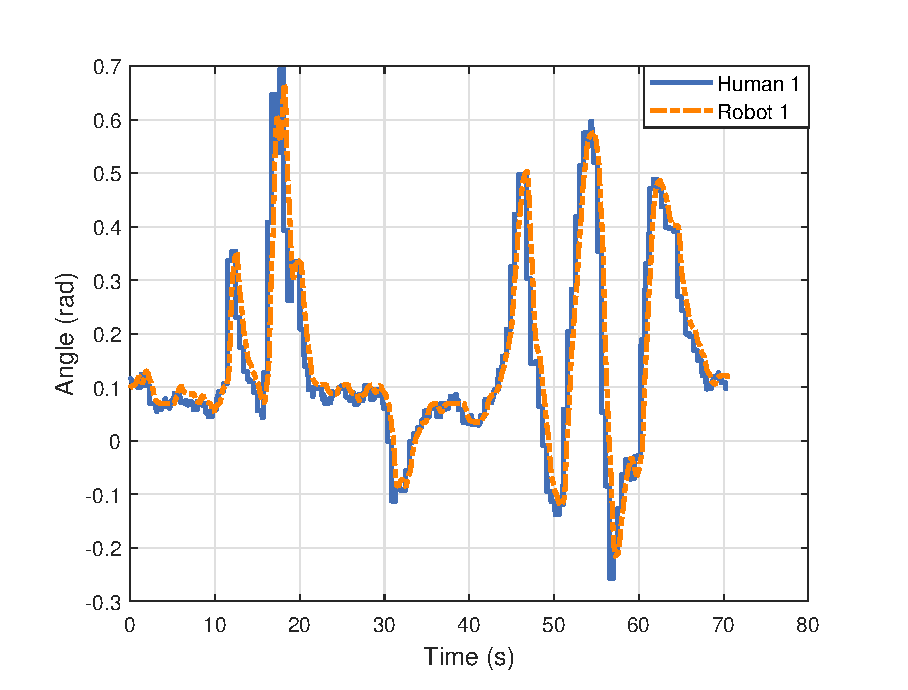
\includegraphics[width=7cm]{figures/chapter3/Fig13a.eps}}
		 \hfill  % 调整两图之间的间距
		\subfloat[\centering]{\includegraphics[width=7cm]{figures/chapter3/Fig13b.eps}}\\
		\subfloat[\centering]{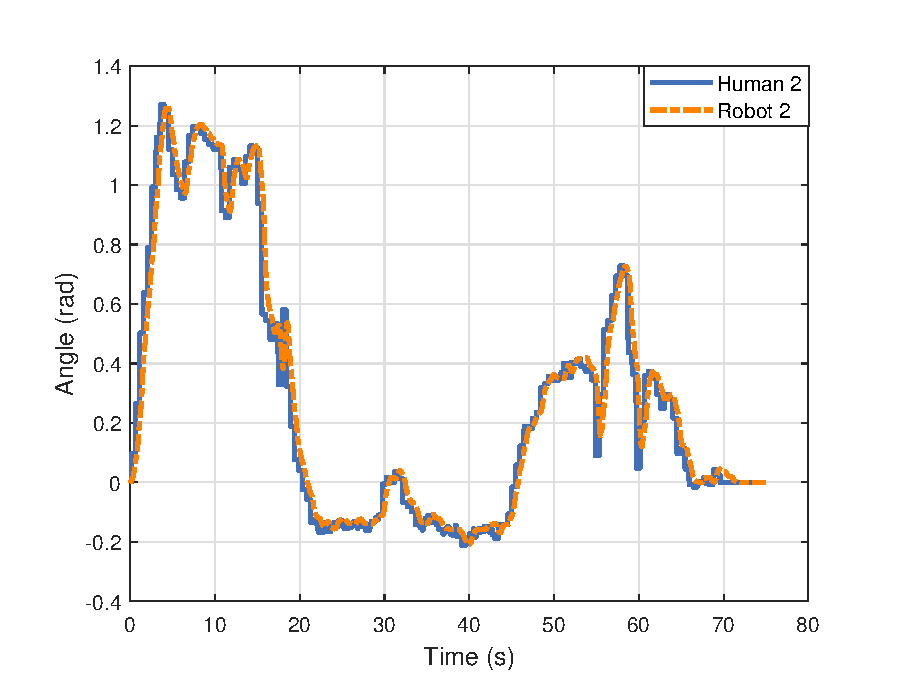
\includegraphics[width=7cm]{figures/chapter3/Fig13c.eps}}
		\hfill  % 调整两图之间的间距
		\subfloat[\centering]{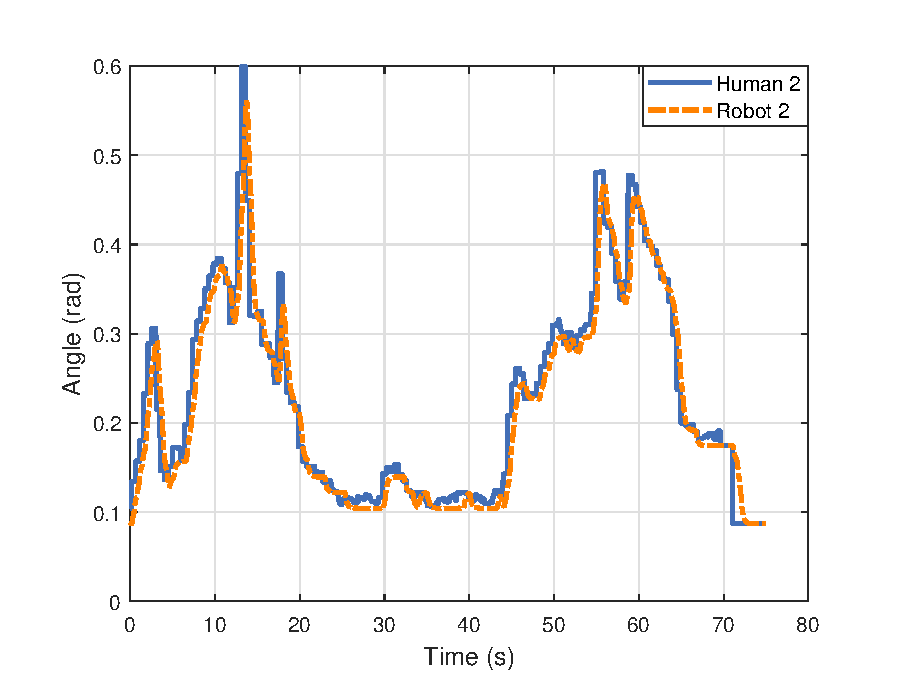
\includegraphics[width=7cm]{figures/chapter3/Fig13d.eps}}
		
	\end{adjustwidth}
\caption{双人动作模仿中左肩屈伸关节和外展-内收关节的轨迹跟踪:(\textbf{a})和(\textbf{b})机器人 1 跟踪表演者 1 左肩屈伸关节和外展-内收关节的关节轨迹;(\textbf{c})和(\textbf{d})机器人 2 跟踪表演者 2 左肩屈伸关节和外展-内收关节的关节轨迹。}

\label{fig:Tracking of Robot Arm Joints dual}
\end{figure} 

\begin{figure}[H]
	\centering
	\begin{adjustwidth}{0cm}{0cm}
		\subfloat[\centering]{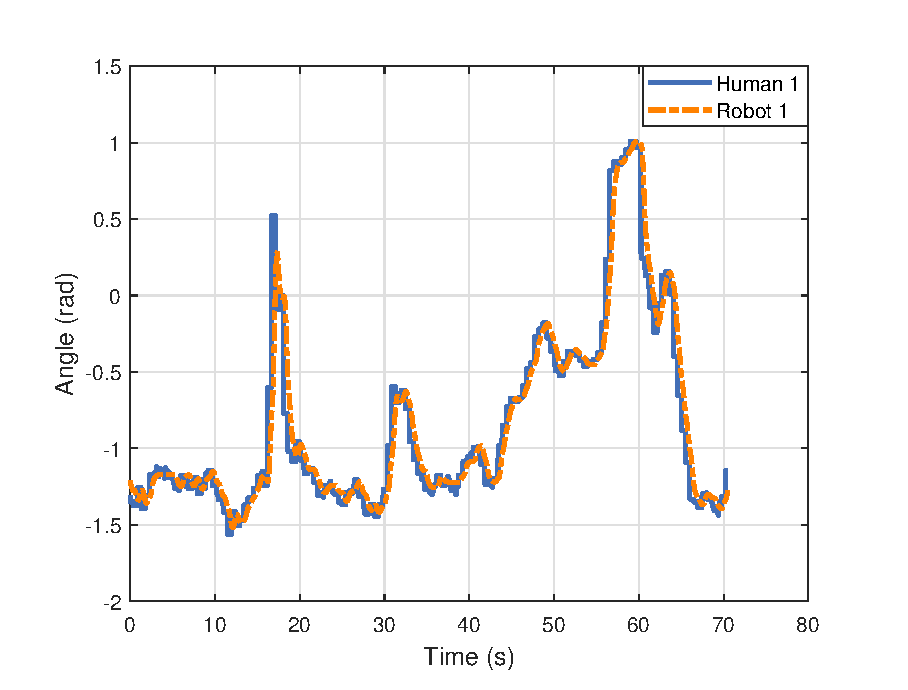
\includegraphics[width=7cm]{figures/chapter3/LSY1.eps}}
		\hfill  % 调整两图之间的间距
		\subfloat[\centering]{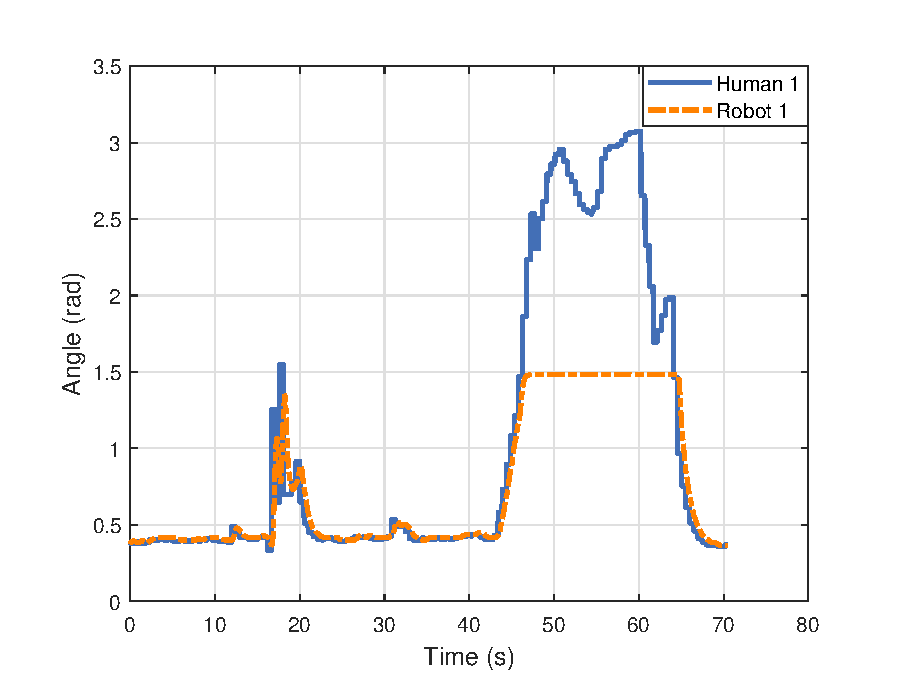
\includegraphics[width=7cm]{figures/chapter3/LE1.eps}}\\
		\subfloat[\centering]{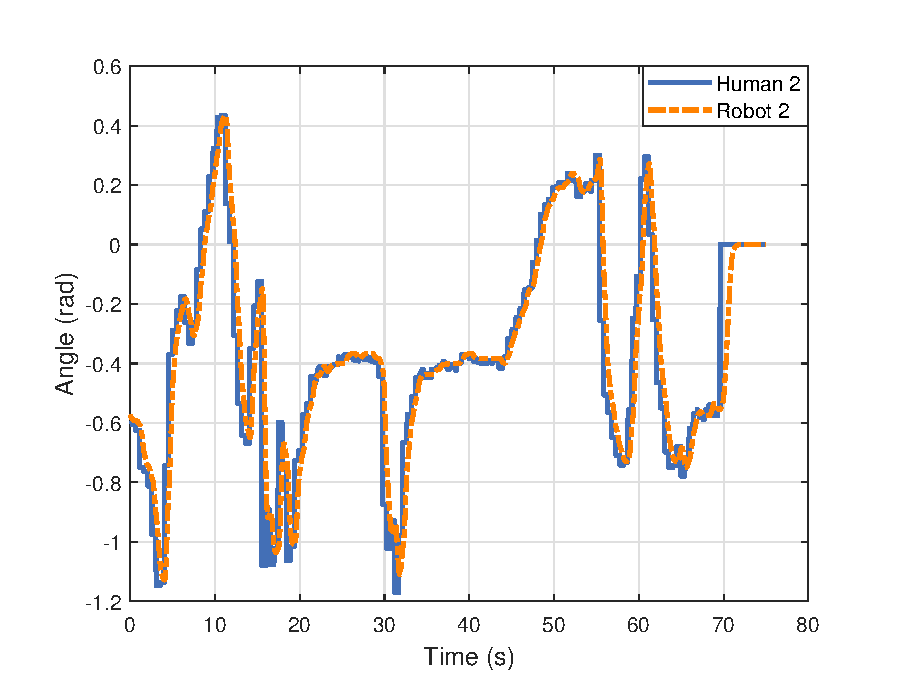
\includegraphics[width=7cm]{figures/chapter3/LSY2.eps}}
		\hfill  % 调整两图之间的间距
		\subfloat[\centering]{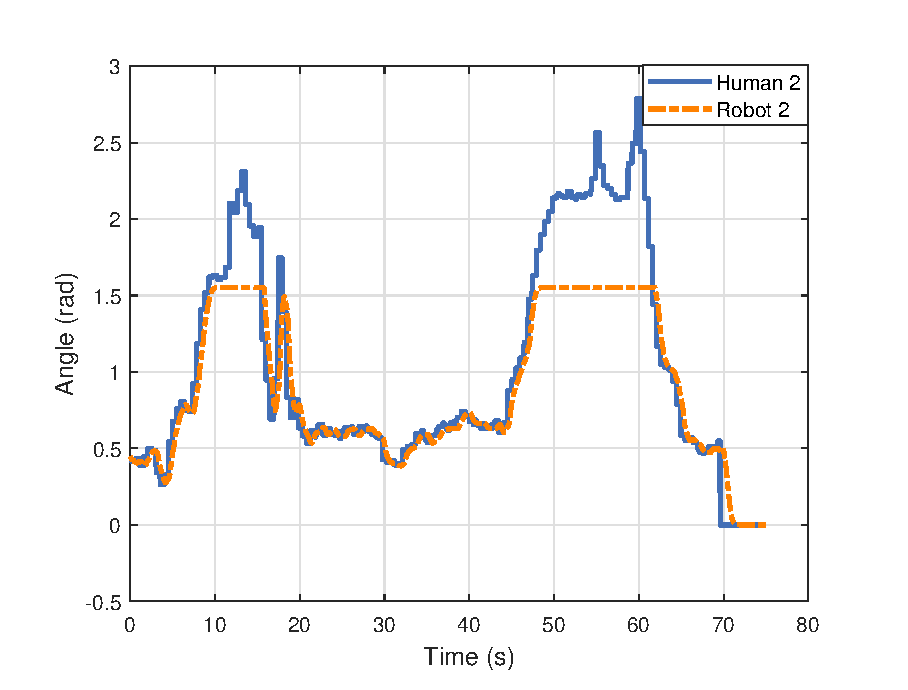
\includegraphics[width=7cm]{figures/chapter3/LE2.eps}}
		
	\end{adjustwidth}
	\caption{双人动作模仿中左肩关节外旋-内旋及肘关节的轨迹跟踪:(\textbf{a})和(\textbf{b})表示机器人 1 跟踪示范者 1 左肩关节外旋-内旋及肘关节的轨迹;(\textbf{c})和(\textbf{d})表示机器人 2 跟踪示范者 2 左肩关节外旋-内旋及肘关节的轨迹。
}
	\label{fig:Robot Arm Joints dual}
\end{figure} 

为了定量评估动作模仿的跟踪性能,本文采用均方误差(Mean Square Error, MSE)作为关节轨迹跟踪精度的指标。MSE 值越小,表示机器人的关节运动越接近目标轨迹。

图 \ref{fig:MSE} 展示了单人和双人动作模仿过程中各关节的均方误差(MSE)。由于关节电机存在固有延迟,跟踪过程中不可避免地引入了误差,从而影响了 MSE 值。结果表明,与单人动作模仿相比,双人动作模仿时各关节的 MSE 并未显著增加,这验证了系统在多智能体动作模仿中的可行性和有效性。此外,肩部外展-内收关节的跟踪 MSE 最小,而肩部内外旋关节的跟踪 MSE 最大。这主要是因为肩部外展-内收的运动特征更为显著,使得从姿态估计输出的人体关键点数据更稳定。因此,通过几何建模计算得到的肩部外展-内收关节参考角波动较小。相比之下,手腕深度信息的波动较大,使得生成的关键点数据变化更明显,导致肩部内外旋关节参考角的波动较大。总之,关节跟踪 MSE 主要来源于姿态估计过程中的数据波动,同时电机响应延迟也会对跟踪精度产生一定影响。
\begin{figure}[H]
	\centering
	\begin{adjustwidth}{0cm}{0cm}
		\subfloat[\centering]{\includegraphics[width=7cm]{figures/chapter3/Fig14_a.eps}}
		\label{fig:MSE_1}
	    \hfill  % 调整两图之间的间距
		\subfloat[\centering]{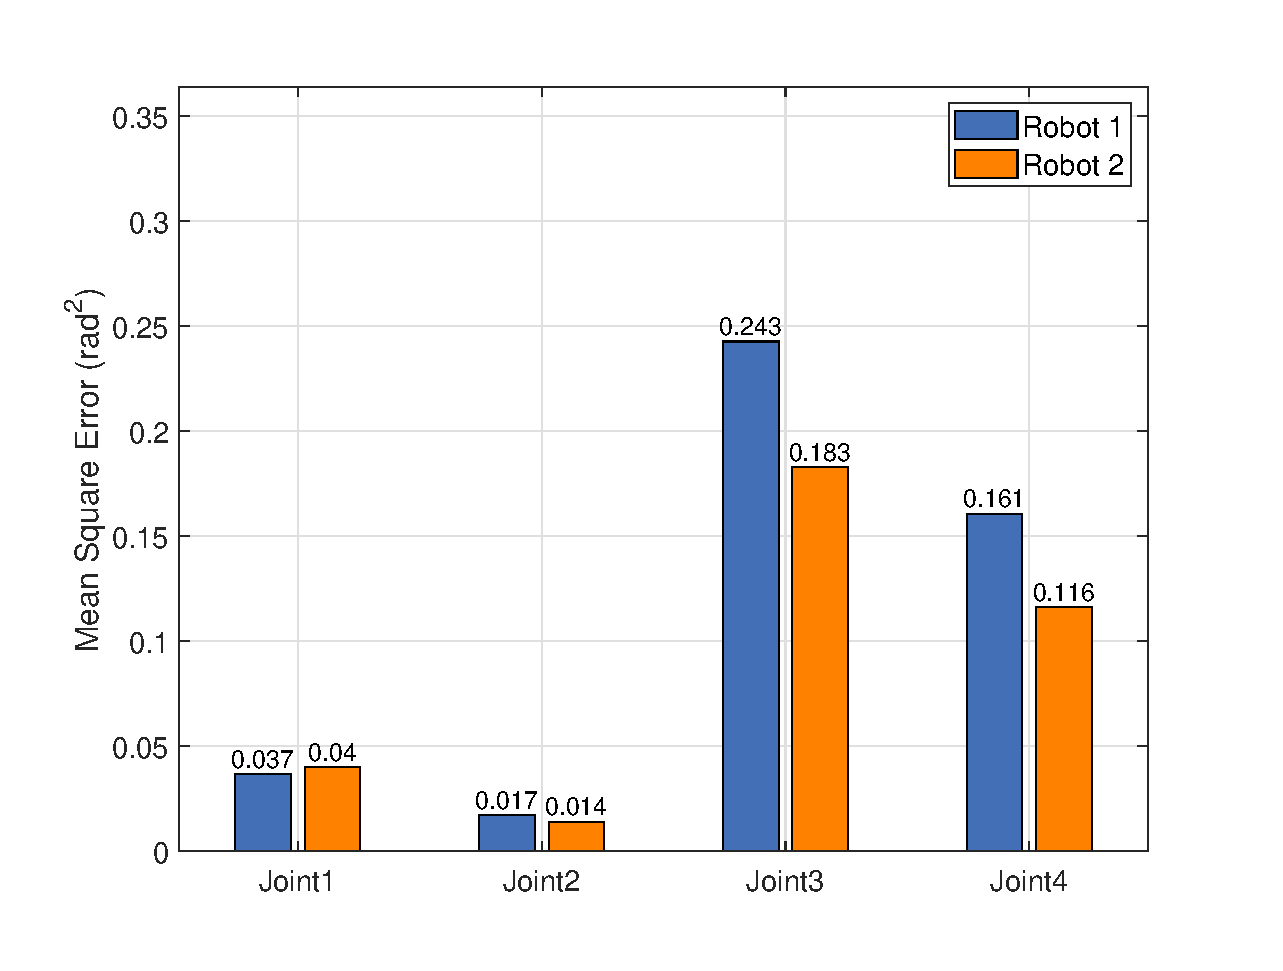
\includegraphics[width=7cm]{figures/chapter3/Fig14_b.eps}}
		\label{fig:MSE_2}
		
	\end{adjustwidth}
\caption{手臂动作模仿过程中关节角度的均方误差(MSE):(\textbf{a})单人手臂动作模仿;(\textbf{b})双人手臂动作模仿。关节 1 对应肩屈伸关节,关节 2 对应肩外展-内收关节,关节 3 对应肩外旋-内旋关节,关节 4 对应肘屈伸关节。}

\label{fig:MSE}
\end{figure} 

\subsection{消融实验}
通过消融实验,我们比较了仅使用几何方法以及基于优化的二次规划(QP)方法在末端执行器位置跟踪任务中的性能。如表~\ref{tab1} 所示,当采用纯几何方法时,末端执行器的跟踪误差为 $9.35 \times 10^{-2}$;而采用 QP 优化方法时,该误差显著降低至 $3.75 \times 10^{-4}$。相比之下,本文提出的方法将末端执行器的跟踪误差进一步降低至 $2.065 \times 10^{-5}$,略高于解析逆向运动学方法,但明显优于几何方法和 QP 方法。


在机器人任务执行中,末端执行器的跟踪精度固然重要,但保持合理的手臂构型同样关键。良好的手臂构型不仅可以避免与环境及机器人自身发生碰撞,还能增强运动的稳定性与安全性。如表 \ref{tab1} 所示,只有本文提出的改进重定向方法在保持可行手臂构型的同时,实现了较小的末端执行器误差。
\begin{table}[ht]
	\centering
	\caption{不同重定向方法的性能比较}
	\begin{tabular}{lcccc}
		\toprule
		方法       & 关节限制 & 构型约束 & 末端执行器误差  & 迭代次数 \\
		\midrule
		几何方法     & $\times$     & \checkmark    & \(9.35 \times 10^{-2}\)    & $\times$   \\
		解析逆运动学 & $\times$     & $\times$      & \(2\times 10^{-6}\)     & 1          \\
		QP方法       & \checkmark   & $\times$      &  \(3.75\times 10^{-4}\) & $\approx100 $      \\
		改进重定向     & \checkmark   & \checkmark    &  \(2.065\times 10^{-5}\)  & $\approx20 $       \\
		\bottomrule
	\end{tabular}
	\label{tab1}
\end{table}

此外,在计算效率方面,所提出的方法仅需约 20 次迭代即可收敛至最优解,相较于传统的基于 QP 的方法,更适合实时应用。

为了直观比较不同重定向方法在动作模仿任务中的表现,我们提供了本文所提出方法的实验视频(\href{https://youtu.be/lXEJFHylUEI}{实验视频}),并在同一关键帧下展示了各重定向方法的差异。如图~\ref{fig:matched_com} 所示,实验结果表明:


基于几何的方法通过追踪肩关节和肘关节角度来保证手臂的配置相似性。然而,由于它并未显式地追踪末端执行器的位置,因此末端执行器的跟踪误差相对较大。逆向运动学(IK)方法能够实现末端执行器位置的跟踪,但由于在求解过程中未考虑关节限制且忽略手臂配置,导致肘关节位置偏差明显,手臂配置相似性降低。QP 方法在优化关节限制的同时能够成功跟踪末端执行器位置,并改善手臂配置。然而,该方法增加了计算复杂度,且手臂配置仍存在一定误差。我们提出的改进重定向方法在保持低末端执行器跟踪误差的同时,能够维持手臂的相似配置,从而提升运动的稳定性和自然性。

为了评估多机器人动作模仿的自然性和可接受性,我们邀请了六名参与者进行示范动作,随后机器人执行模仿及任务操作。评价指标如下:
1. **动作平滑性 (Motion Smoothness, MS)**:评估机器人执行过程中是否存在不连续或突兀的动作。
2. **姿态可行性 (Pose Feasibility, PF)**:评估机器人手臂姿态是否与人类示范者保持相似。
3. **任务完成度 (Task Achievement, TA)**:评估机器人是否准确完成指定的模仿任务。
4. **总体用户偏好 (Overall User Preference)**:反映参与者对整体模仿质量的主观评价。

 用户评分采用1(差)到5(优)的五分制,统计结果如表 \ref{tab2} 所示。实验结果表明,在所有评价指标上,我们的方法均优于基于几何方法(geometry-based)、逆向运动学(IK)和二次规划(QP)方法。尤其在动作平滑性和姿态可行性方面,用户主观评分明显更高。这表明,改进的重定向方法不仅提高了模仿精度,同时也增强了动作的自然性和用户可接受性。

 \subsection{局限}
 所提出的改进重定向算法能够有效地计算出最优关节角,同时满足手臂几何结构一致性和末端执行器位置跟踪的要求。通过结合多人人体姿态估计技术,该框架实现了多机械臂的动作模仿与协作任务,增强了系统的适应性和多任务处理能力。尽管人体运动运动学长期以来一直是研究前沿,但本研究在重定向算法方面相较于现有方法取得了进展。尤其是,将改进的重定向算法与多机器人协作任务相结合,并利用实时人体姿态估计进行机器人动作模仿,本方法在复杂环境中显著提升了动作模仿的精度与协调性。
 然而,所提出的框架仍存在一定局限性,尤其是在姿态方向跟踪方面。由于我们的姿态估计系统主要通过单目相机估计末端执行器的位置,它只能获取位置数据,而无法完整提取关节的全姿态信息(包括旋转分量)。这一限制显著影响了关节运动的灵活性,尤其是在涉及前臂旋前-旋后和手腕屈伸等复杂动作时,机器人无法充分调整这些关节以满足任务要求。未来的研究可以引入完整的姿态估计,实现位置与方向的综合跟踪,从而提升机器人在复杂任务中的灵活性与精度。关于关节限位约束,如图 \ref{fig:Robot Arm Joints dual} (b) 和 (d) 所示,无法实现精确跟踪主要是由于机械结构限制了关节运动范围,这一问题在传统控制方法中同样存在。为解决该局限性,未来工作可引入更加灵活的自适应关节限位控制策略,使机器人在不超出机械极限的前提下调整运动范围,从而减轻关节限位带来的影响。

\begin{figure}[h]
	\centering
	\begin{minipage}{0.48\linewidth}
		\centering
		\captionof{table}{不同重定向方法的用户主观评价}
		\begin{tabular}{lcccc}
			\toprule
			方法  & MS  & PF  & TA  & 综合评分 \\
			\midrule
			几何方法     & 4   & 5   & 2   & 4   \\ 
			逆运动学方法 & 4   & 2   & 3   & 2   \\
			QP 方法      & 3   & 3   & 3   & 3   \\
			本文方法     & 5   & 5   & 4   & 5   \\
			\bottomrule
		\end{tabular}
		\label{tab:user_evaluation}
	\end{minipage}
	\hfill
	\begin{minipage}{0.5\linewidth}
		\centering
		\includegraphics[width=\linewidth]{figures/chapter3/mathed_com.png}
		\caption{相同动作关键帧下不同重定向方法的对比结果。橙色点表示目标位置,蓝色点表示实际到达位置。}
		\label{fig:matched_comparison}
	\end{minipage}
\end{figure}

\section{结论}
本文提出了一个综合性的实时多仿人机器人手臂动作模仿框架,该框架采用改进的重定向方法,有效实现了手臂运动学配置与末端执行器精度之间的最佳平衡。通过整合多人人体姿态估计技术,该框架不仅支持多仿人机器人之间的协作运动,还为复杂任务中的多机器人协作提供了有效解决方案。

实验结果表明,机器人能够成功复现各种人类手臂动作。尽管随着示范者数量的增加,姿态估计误差有所上升,但整体动作模仿仍保持较高的跟踪精度和末端执行器准确性。此外,在倒水、物品分类及协作等任务中,我们进一步验证了改进重定向方法在保持手臂运动学结构完整性和末端执行器精度方面的优越性能。此外,随着多人人体姿态估计技术的整合,即使检测对象数量增加,系统仍能保持良好的实时性能,有效避免了计算负载的大幅增加。

尽管该框架在高精度与高效率方面表现出色,但在姿态跟踪上仍存在一定局限性。未来的研究将重点进一步优化姿态估计技术,实现位置与姿态的综合跟踪,从而提升机器人在复杂任务中的灵活性与精度,并使其在多智能体交互与协作任务中发挥更大作用。
%    \chapter{基于模仿学习的全身控制框架}
大规模动作捕捉数据集涵盖了从风格化行走到复杂全身行为在内的多样化、高动态运动模式。若能够将这些人类运动有效迁移至类人机器人,它们将形成一套可复用的运动基元库,从而为多种下游任务提供统一且具有良好泛化能力的控制基础。

类人机器人由于其与人体高度相似的结构和丰富的自由度,天然适合执行这类全身运动并参与人机物理交互。然而,这种结构相似性也使其控制问题远比传统机器人更加复杂:高维状态空间、强关节耦合以及不稳定的接触动力学共同构成了严峻挑战,从而显著制约了这些人类动作在真实机器人上的直接落地。

提升学习型控制器性能的一条自然途径是引入动作捕捉数据或人工设计的动画数据作为运动先验。现有研究通常采用一种分层控制结构,即在运动学动画系统之上叠加一个基于物理的跟踪控制器 \cite{lee2010data}。然而,该类方法存在显著局限性:一方面,运动学层必须生成物理上可被精确跟踪的参考轨迹,否则会导致控制失败或运动质量下降;另一方面,所得的物理控制器在偏离原始参考以实现自恢复或任务导向行为时缺乏足够的灵活性。此外,这类系统在工程实现上通常较为复杂,难以扩展到大规模、多样化动作集。

近年来,基于物理的角色动画研究 \cite{luo2023universal,tessler2024maskedmimic,huang2025diffuse,pan2025tokenhsi} 在将人类动作合成为面向下游任务的动态全身控制策略方面取得了显著进展。然而,这些成果主要建立在仿真环境中,其中智能体通常假设拥有理想化动力学、无限执行能力以及完美的状态观测,这与真实世界中的类人机器人存在本质差异。真实机器人必须面对未建模动力学、执行器与传感器限制以及不完备状态估计等问题,使得直接迁移这些方法往往难以获得稳定可靠的表现。因此,要在真实硬件平台上实现类似水平的运动能力,仍然缺乏两个关键要素:(1)一种可扩展且高质量的运动跟踪框架,能够将运动学参考动作转化为鲁棒且高度动态的真实机器人运动,同时避免传统方法中常见的过度随机化、抖动与运动质量退化问题;(2)一种有效的训练动作采样机制,能够在复杂动作与简单动作之间合理分配训练资源,避免由于难度分布不均导致的泛化性能下降。

针对上述挑战,本文提出了一种面向真实世界的类人机器人全身动作学习框架。该框架首先构建了一条高精度的运动跟踪流水线,使机器人能够在真实硬件上以接近动画级质量执行包括摔倒爬起、坐下起身等在内的高度动态全身动作。与仅进行表观模仿的方法不同,该框架在学习过程中显式建模物理约束与动力学一致性,从而有效抑制了以往深度强化学习方法(如 \cite{duan2016benchmarking})中常见的滑移、抖动与姿态漂移等运动伪影。在存在外界扰动或对原始动作进行修改时,所生成的运动仍保持自然流畅,且恢复策略表现出高度鲁棒性,无需依赖复杂的人工工程化调节。

\section{相关工作}

类人机器人的物理交互本身具有高度挑战性,其中一个根本原因在于系统动力学的强非线性和高维耦合特性。传统控制方法通常依赖精确的动力学建模与解析控制策略 \cite{chignoli2021humanoid,dallard2023synchronized,sentis2018whole,ramos2019dynamic},然而在涉及复杂接触与全身协调的场景中,这类方法往往难以兼顾稳定性与灵活性。

近年来,随着强化学习(Reinforcement Learning, RL)和仿真到真实(sim-to-real)迁移技术的快速发展,四足机器人和类人机器人在学习复杂全身技能方面取得了显著进展,尤其在高复杂度和强接触任务中展现出卓越的适应能力与运动性能 \cite{agarwal2023legged,cheng2024extreme,duan2024learning,fu2023deep,ito2022efficient,jeon2023learning,ji2023dribblebot}。这些成果表明,基于数据驱动的方法能够有效缓解精确建模带来的局限。

在类人机器人领域,一些研究进一步将 RL 应用于全身控制与动作生成 \cite{cheng2024expressive,fu2024humanplus},尝试提升机器人的动作表现力并支持操作与模仿学习等任务。尽管这些方法已在一定程度上实现了更自然的运动风格,但在动作多样性与机动性方面仍存在明显限制,表明其尚难全面覆盖真实世界中丰富多变的运动需求。

与此相对应,RL 在计算机图形学与虚拟角色控制领域已经展现出极强的动作生成能力,例如在人体动作模仿 \cite{peng2018deepmimic}、多任务技能学习 \cite{peng2022ase} 以及基于视觉输入的人体动作跟踪 \cite{18} 等方面均取得了显著成功。同时,在真实硬件平台上,RL 也已被用于实现稳定而灵活的双足行走 \cite{radosavovic2023learning,siekmann2021blind},进一步验证了其在高维动力学控制问题中的潜力。

然而,纯强化学习方法通常依赖复杂的奖励设计和精细的超参数调节,在面对多样化动作和任务需求时,训练代价高昂且可扩展性受限。为缓解这一问题,将 RL 与人体运动数据作为先验知识相结合已成为一种有效范式。例如,H2O \cite{he2024learning} 通过将 RL 与遥操作示例相结合,实现了全尺寸类人机器人的全身控制,而 OmniH2O \cite{he2024omnih2o} 进一步引入多种控制接口,以支持更加复杂和多样化的交互任务。

在动作表现力方面,ExPressive \cite{cheng2024expressive} 通过 RL 学习下肢行走策略,并结合上肢运动跟踪,实现了上半身模仿与下半身运动控制的协同。然而,这类依赖示例数据的动作跟踪方法受限于动作捕捉数据的获取成本与规模,在真实类人机器人硬件上实现同时具备**高运动质量**与**高度动态技能支持**的多动作跟踪尚未被成功展示。本节旨在填补这一空白,通过跟踪包含多种风格与难度、持续数分钟的人类参考动作序列,实现多样化、高动态的人形机器人运动复现。


\section{方法}
我们将类人机器人的全身运动控制建模为一个\emph{目标条件化(goal-conditioned)}的策略学习问题,其策略形式化表示为
$\pi : G \times S \rightarrow A ,$
其中 $G$ 表示用于描述期望行为的目标空间,$S$ 为观测空间,$A$ 为动作空间,对应机器人关节的控制指令(如关节位置或力矩)。在本文其余部分中,在不失一般性的前提下,我们基于 Droid 类人机器人平台对观测空间与动作空间进行具体定义。需要指出的是,所提出的方法同样适用于具有相似身体结构、但在自由度数量或驱动形式上有所差异的类人机器人系统。




\subsection{运动跟踪目标}
我们从经重定向处理后的参考动作出发,该动作由一系列广义位置和速度关键帧 $(\mathbf{q}_m, \mathbf{v}_m)$ 表示。通过正向运动学,对于每一个刚体 $b \in \mathcal{B}$,可以计算其对应的位姿 $T_{b,m}$ 以及空间速度(twist)$V_{b,m}$,其中 $\mathcal{B}$ 表示机器人所有刚体的集合。

在真实硬件执行过程中,由于外部扰动以及仿真到现实(sim-to-real)差异的存在,参考动作在全局坐标系下往往会产生不可避免的漂移。为了在允许一定全局偏移的同时保持动作的相对结构与风格,控制器不应直接跟踪所有刚体的绝对位姿。

为此,我们选取一个锚定刚体 $b_{\text{anchor}} \in \mathcal{B}$(通常为根部或躯干),并将参考动作重新锚定到该刚体的期望状态上。具体而言,对于锚定刚体,直接采用参考动作中的位姿,即 $\hat{T}_{b_{\text{anchor}}} = T_{b_{\text{anchor}},m}$。

对于其余刚体 $b \in \mathcal{B} \setminus \{b_{\text{anchor}}\}$,其期望位姿定义为 $\hat{T}_b = T_\Delta \, T^{-1}_{b_{\text{anchor}},m} \, T_{b,m}$,其中对齐变换 $T_\Delta = (p_\Delta, R_\Delta)$,并满足
$p_\Delta = [p_{b_{\text{anchor}}}.x,\ p_{b_{\text{anchor}}}.y,\ p_{b_{\text{anchor}}}.z_m]$,
以及
$R_\Delta = R_z\!\left(\mathrm{yaw}\!\left(R_{b_{\text{anchor}}} R^{\top}_{b_{\text{anchor}},m}\right)\right)$。

该对齐变换在保持身体高度不变的同时,对齐参考动作与当前机器人的偏航角,并将参考动作的平面位置映射至机器人下方,从而将全局参考动作转化为局部可执行的跟踪目标。

对于空间速度,我们直接采用参考动作中的速度信息,即对所有 $b \in \mathcal{B}$,有 $\hat{V}_b = V_{b,m}$。

由于机器人包含大量空间位置相近的刚体,对所有刚体进行跟踪既计算开销较大,也缺乏必要性。因此,我们选取一个用于运动约束的目标刚体子集 $\mathcal{B}_{\text{target}} \subseteq \mathcal{B}$,并将最终的运动跟踪目标定义为
$g_{\text{tracking}} = \{\hat{T}_{b_{\text{anchor}}},\ \hat{T}_b,\ \hat{V}_b\},\ \forall b \in \mathcal{B}_{\text{target}}$。

\subsection{观测}
我们将策略的观测空间拆解为一个单时间步向量,由以下两个部分组成。
\textbf{(1) 参考相位信息。}
参考相位。我们引入参考动作中的关节位置和关节速度$c = [q_{\text{joint},m}, \, v_{\text{joint},m}],$
该信息仅用于提供相位参考,策略并不被要求直接跟踪这些关节数值。

\textbf{(2) 本体感知信息。}
其他本体感知信息。我们进一步包含机器人在根坐标系下根节点的重力投影 $g_t \in \mathbb{R}^3$、根节点角速度 $\omega_t \in \mathbb{R}^3$,以及关节位置 $q_{\text{joint}}$、关节速度 $v_{\text{joint}}$,和上一时刻的动作 $a_{\text{last}}$。

综合上述各项,完整的观测向量表示为
\begin{equation}
    o = [c,\;g_t,\;\omega_t,\; q_{\text{joint}},\; v_{\text{joint}},\; a_{\text{last}} ].
\end{equation}
以上观测能够避免了一般学习任务中需要依靠状态估计,估计出线速度相关分量以及计算出锚点的位置,重而降低观测复杂性。

\subsection{奖励设计}
我们以一种简单、直观且具有通用性的方式设计奖励函数,其由两部分组成:(1) 任务奖励,作为正向奖励,采用统一权重并在任务空间中定义;(2) 最小化的正则化惩罚项,用于避免对跟踪性能造成负面影响。任务奖励由身体跟踪奖励构成。首先,针对每一个目标刚体 $b \in B_{\text{target}}$,基于期望的位姿与速度 $(\hat{T}_b, \hat{V}_b)$ 以及实际的位姿与速度 $(T_b, V_b)$ 计算误差度量:位置误差 $e_{p,b} = \hat{p}_b - p_b$,姿态误差 $e_{R,b} = \log(\hat{R}_b R_b^\top)$,线速度误差 $e_{v,b} = \hat{v}_b - v_b$,以及角速度误差 $e_{w,b} \approx \hat{w}_b - w_b$(在姿态误差较小的假设下)。随后,在所有目标刚体上计算各类误差的均方值:$\bar{e}_\chi = \frac{1}{|B_{\text{target}}|} \sum_{b \in B_{\text{target}}} \| e_{\chi,b} \|^2$,其中 $\chi \in \{p, R, v, w\}$。每一种误差度量随后通过高斯形式的指数函数进行归一化:$r(\bar{e}_\chi, \sigma_\chi) = \exp\!\left(-\bar{e}_\chi / \sigma_\chi^2\right)$,其中 $\sigma_\chi$ 为通过经验确定的名义误差尺度。综合后的任务奖励定义为:$r_{\text{task}} = \sum_{\chi \in \{p, R, v, w\}} r(\bar{e}_\chi, \sigma_\chi)$。在正则化方面,我们仅引入对仿真到真实迁移至关重要的三个惩罚项。其中,关节限位惩罚 $r_{\text{limit}}$ 用于鼓励关节位置保持在软限位范围内;动作变化率惩罚 $r_{\text{smooth}}$ 用于鼓励相邻时间步的动作平滑变化,从而避免策略产生过度抖动;自碰撞惩罚 $r_{\text{contact}}$ 通过统计自接触力超过预设阈值的刚体数量来计算,该统计在 $b \notin B_{\text{ee}} \subseteq B$ 的刚体集合上进行,其中 $B_{\text{ee}}$ 表示末端执行器刚体集合。最终的总奖励形式为:$r = r_{\text{task}} - \lambda_l r_{\text{limit}} - \lambda_s r_{\text{smooth}} - \lambda_c r_{\text{contact}}$,其中 $\lambda_l, \lambda_s, \lambda_c > 0$ 为各正则化项对应的权重系数。作为可选项,还可以为锚定刚体 $b_{\text{anchor}}$ 添加一个全局跟踪奖励,其结构与 $r_{\text{tracking}}$ 相同,但仅使用位置误差 $e_{p,b_{\text{anchor}}}$ 和姿态误差 $e_{R,b_{\text{anchor}}}$ 来计算。

\subsection{难度采样}
训练包含长时间序列的运动时不可避免地会面临一个问题:不同时间段的难度并不均衡。因此,像以往工作 \cite{14,34,17} 中常用的那样,对整条轨迹进行均匀采样,往往会对简单片段过度采样、而对困难片段采样不足,从而导致奖励方差增大并降低训练效率。基于这一观察,一个自然的想法是更加频繁地从困难区域进行采样。为此,我们将整段运动轨迹的起始索引划分为 $S$ 个 bin,每个 bin 对应 1 秒的时间长度,并根据经验性的失败统计信息对这些 bin 进行采样。设 $N_s$ 和 $F_s$ 分别表示从第 $s$ 个 bin 开始的回合数和失败次数。为防止由于短期波动导致采样概率出现离散跳变,我们对失败率采用指数滑动平均进行时间平滑处理。考虑到失败更可能由终止前不久采取的次优动作引起,我们进一步对失败率施加一个非因果卷积,并使用指数衰减核 $k(u)=\gamma^u$(其中 $\gamma$ 为衰减系数),以便对更接近当前时刻的失败赋予更大的权重。最终,从第 $s$ 个 bin 进行采样的概率定义为
\[
p_s=\frac{\sum_{u=0}^{K-1}\alpha^u \bar r_{s+u}}{\sum_{j=1}^{S}\sum_{u=0}^{K-1}\alpha^u \bar r_{j+u}},
\]
其中 $\bar r_s$ 表示第 $s$ 个 bin 的平滑失败率。为了在优先关注困难片段的同时保持对简单片段的覆盖,并缓解灾难性遗忘问题,我们将上述概率 $p_s$ 与均匀分布进行混合,得到 $p'_s=\lambda\frac{1}{S}+(1-\lambda)p_s$,其中 $\lambda$ 为均匀采样比例。最终,起始 bin 从多项分布 $\text{Multinomial}(p'_1,\ldots,p'_S)$ 中采样,从而在整体训练过程中优先覆盖更具挑战性的区域。

\section{讨论}
本节通过仿真以及在 Droid 人形机器人上的真实世界部署,对所提出的运动控制框架进行了实验验证,结果表明该方法能够对全身动作进行高鲁棒和精准跟踪。需要说明的是,在本节中,我们对所有策略均使用同一组超参数进行训练。

% \subsection{Sim-to-Sim 性能评估}
我们使用由 Unitree 重定向的 LAFAN1 数据集~\cite{harvey2020robust},该数据集包含多种敏捷且多样的人体运动,例如冲刺、转身跳跃和爬行,同时还包含来自先前工作~\cite{zhang2025hub,he2025asap} 的短时单动作片段。LAFAN1 数据集包含 40 条时长为数分钟的参考序列,每一条都属于一个较大的动作类别,并在该类别下包含多种不同的具体动作。我们从中随机选择了 25 条参考序列,并确保每个类别至少包含一条。实验结果表明,在 sim-to-sim 评估中,这些参考序列均能够完整执行。由于测试场地空间受限,我们进一步从这些参考序列中有意挑选了 29 条具有挑战性的动作片段,这些片段包含高度动态且接触频繁的行为,并将其部署到真实硬件上,以评估 sim-to-real 的迁移性能。所有用于 sim-to-sim 以及 sim-to-real 评估的动作列表详见表~I。


\subsection{基线方法}
为系统评估所提出方法的有效性与设计选择的合理性,我们选取以下两类典型设置作为对比基线。

\subsubsection{不同跟踪目标}
在运动跟踪任务中,跟踪目标的表示形式对于实现稳定且可靠的仿真到现实(sim-to-real)迁移至关重要。一种常见选择是采用局部关节空间表示进行跟踪,该表示具有维度低、结构紧凑以及计算效率高等优点,因此在实时控制系统中具有较强的实用性。然而,关节空间表示难以直接刻画末端或身体关键部位在笛卡尔空间中的几何约束。

相比之下,直接对机器人各身体部位的空间位姿进行跟踪能够在笛卡尔空间中提供明确的几何约束,有助于保持整体动作结构与空间一致性。但该方式通常需要更高维度的状态表示,并引入更大的模型规模和更高的推理开销,从而对实时性能提出更高要求。上述两种跟踪目标在计算效率与空间可解释性之间形成了一种权衡关系,由此引出了一个关键问题:哪一种跟踪目标形式更有利于实现高质量的 sim-to-real 迁移。

为回答这一研究问题,我们对两种不同的状态表示方式进行了对比分析,具体如下:

\begin{itemize}
    \item \textbf{Body-Pos State:}
    \begin{itemize}
        \item \textbf{全局状态(Global States):} 根节点位置($\mathbb{R}^3$)、线速度($\mathbb{R}^3$),以及以旋转向量形式表示的朝向($\mathbb{R}^3$),均相对于当前时刻的角色坐标系表示。
        \item \textbf{局部状态(Local States):} 所有刚体在角色坐标系下的笛卡尔位置($\mathbb{R}^{3B}$)及其线速度($\mathbb{R}^{3B}$),其中 $B$ 表示刚体数量。
    \end{itemize}

    \item \textbf{Joint-Pos State:}
    \begin{itemize}
        \item \textbf{全局状态(Global States):} 与 Body-Pos State 相同,包括根节点位置、线速度及旋转向量形式的朝向。
        \item \textbf{局部状态(Local States):} 关节角度($\mathbb{R}^{J}$)及关节角速度($\mathbb{R}^{J}$),其中 $J$ 表示关节数量。
    \end{itemize}
\end{itemize}

表~\ref{tab:state_ablation} 总结了两种状态表示在两类任务(行走+扰动与舞蹈+扰动)中的成功率表现。实验结果表明,\textbf{Body-Pos 状态表示在两项任务中均显著优于 Joint-Pos 表示}。

\begin{table}[t]
\centering
\caption{不同状态表示在不同任务下的成功率对比}
\label{tab:state_ablation}
\begin{tabular}{lcc}
\toprule
\textbf{状态表示} & \textbf{行走+扰动} & \textbf{舞蹈+扰动} \\
\midrule
Body-Pos State  & 100\% & 90\% \\
Joint-Pos State & 70\%  & 0\%  \\
\bottomrule
\end{tabular}
\end{table}

尽管从理论上看,基于关节角度的表示更符合 Markov 性假设,但在实际应用中,关节位置估计中的微小误差会沿运动学链逐级累积,使得该表示方式在扩散预测过程中更容易产生误差放大。相比之下,直接预测笛卡尔空间中的身体位姿能够有效缓解该问题,从而表现出更高的稳定性与鲁棒性。


\subsubsection{不同观测设计}
观测空间的设计在强化学习训练过程中同样起着决定性作用,其直接影响策略的学习效率与任务成功率。在确定跟踪目标之后,是否引入历史观测信息、以及是否对参考动作进行前瞻预测,都会显著影响策略网络的表达能力与泛化性能。

为此,我们设计并比较了以下三种典型观测配置:
(1)不使用任何历史信息,仅采用单时刻观测;
(2)对参考动作进行 $5$ 帧的前瞻预测,同时对机器人本体感觉信息采用历史堆叠;
(3)对所有观测量(包括参考动作与本体感觉信息)均采用历史堆叠。

通过上述基线设置的对比实验,我们系统分析不同观测设计对学习稳定性、跟踪精度以及 sim-to-real 迁移性能的影响。

进一步地,我们对不同观测历史设计方式进行了消融分析,具体包括:
\begin{enumerate}
    \item \textbf{无历史信息:} 所有观测仅使用当前时刻信息;
    \item \textbf{参考预测 + 本体历史堆叠:} 对参考动作预测未来 $5$ 帧,本体状态采用历史堆叠;
    \item \textbf{统一历史堆叠:} 所有观测(参考动作与本体状态)均采用历史堆叠。
\end{enumerate}

表~\ref{tab:history_ablation} 给出了不同观测设计下的训练稳定性与收敛特性。

\begin{table}[t]
\centering
\caption{不同观测历史设计的训练稳定性对比}
\label{tab:history_ablation}
\begin{tabular}{lccc}
\toprule
\textbf{观测方式} & \textbf{迭代次数} & \textbf{Loss 爆炸} \\
\midrule
无历史信息 & 12000 & 否 \\
参考预测 + 本体历史堆叠 & 4000 & 是 \\
统一历史堆叠 & 8000 & 否 \\
\bottomrule
\end{tabular}
\end{table}

从表中可以看出,统一采用历史堆叠的方式虽然在收敛速度上不及使用参考预测的方法,但其训练过程更加稳定。相比之下,引入参考动作预测虽然能够加快早期学习速度,但容易导致策略过拟合,从而使训练过程中的损失函数迅速增大,最终导致学习失败。

另一方面,相较于不使用历史信息的设置,历史堆叠能够使策略显式建模时间相关性,从而提升对动力学不确定性和观测噪声的鲁棒性,这对于 sim-to-real 迁移尤为重要。

\subsection{评价指标}
我们将我们的方法与其他全身控制方法进行对比,包括ASAP,PBHC,H2O等,为了更好的说明效果,我们定义一下评价指标
成功率:我们报告策略的 \textbf{成功率(success rate)},当在任意时刻机器人平均身体部位距离误差超过 $0.5\,\mathrm{m}$ 时,认为该次模仿任务失败。

此外,我们通过以下指标评估策略对参考运动的跟踪能力:
\begin{itemize}
    \item 全局平均刚体位置误差 $E_{\text{g-mpdpe}}$(mm);
    \item 相对于根节点的平均刚体位置误差 $E_{\text{mpdpe}}$(mm);
    \item 加速度误差 $E_{\text{acc}}$(mm/frame$^2$);
    \item 根节点速度误差 $E_{\text{vel}}$(mm/frame)。
\end{itemize}

全局平均刚体位置误差用于衡量各刚体在\textbf{全局坐标系}下的平均位置偏差,其定义为:
\begin{equation}
E_{\text{g-mpbpe}} = \mathbb{E}\Big[ \big\| \mathbf{p}_t - \mathbf{p}^{\text{ref}}_t \big\|_2^2 \Big],
\label{eq:eg-mpbpe}
\end{equation}
其中 $\mathbf{p}_t$ 表示当前时刻各刚体在全局坐标系下的位置,$\mathbf{p}^{\text{ref}}_t$ 表示对应的参考刚体位置。

相对于根节点的平均刚体位置误差用于衡量在\textbf{根节点坐标系}下的刚体位置偏差,其定义为:
\begin{equation}
E_{\text{mpbpe}} = \mathbb{E}\Big[ 
\big\| (\mathbf{p}_t - \mathbf{p}_{\text{root},t}) - (\mathbf{p}^{\text{ref}}_t - \mathbf{p}^{\text{ref}}_{\text{root},t}) \big\|_2^2
\Big],
\label{eq:empbpe}
\end{equation}
其中 $\mathbf{p}_{\text{root},t}$ 和 $\mathbf{p}^{\text{ref}}_{\text{root},t}$ 分别表示当前运动与参考运动在时刻 $t$ 的根节点位置。


上述指标的最终结果均在所有测试运动序列上取平均值。

\begin{table*}[t]
\centering
\caption{不同方法在不同难度等级下的性能对比结果(均值 $\pm$ 标准差,$\downarrow$ 表示越小越好)}
\label{tab:main_results_cn}
\resizebox{\textwidth}{!}{
\begin{tabular}{lccccc}
\toprule
\textbf{难度} &
$\mathbf{Succ\uparrow}$ &
$\mathbf{E_{g_{mpbpe}}\downarrow}$ &
$\mathbf{E_{mpdpe}\downarrow}$ &
$\mathbf{E_{acc}\downarrow}$ &
$\mathbf{E_{vel}\downarrow}$ \\
\midrule
\multicolumn{6}{l}{\textbf{简单}} \\
\midrule
OmniH2O  & 92$\pm$0.00 & 233.54$\pm$4.013 & 103.67$\pm$1.912 & 4.50$\pm$0.0228 & 5.56$\pm$0.031 \\
ASAP & 97$\pm$0.00 & 108$\pm$0.678 & 49.4$\pm$0.49 & 2.74$\pm$0.025 & 4.46$\pm$0.020 \\
PBHC & 99$\pm$0.00 & 53.25$\pm$17.60 & 46.4$\pm$0.269 & 2.63$\pm$0.012 & 4.59$\pm$0.021 \\
Ours & 100$\pm$0.00 & 41.79$\pm$1.71 & 21.86$\pm$2.0 & 2.35$\pm$0.017 & 4.23$\pm$0.031 \\
\midrule
\multicolumn{6}{l}{\textbf{中等}} \\
\midrule
OmniH2O  & 85$\pm$0.00 & 433.64$\pm$16.22 & 151.42$\pm$7.340 & 4.83$\pm$0.02 & 5.69$\pm$0.019 \\
ASAP & 96$\pm$0.00 & 126.48$\pm$27.01 & 48.87$\pm$7.550 & 2.53$\pm$0.019 & 4.45$\pm$0.026 \\
PBHC & 98$\pm$0.00 & 120.57$\pm$17.01 & 36.05$\pm$4.150 & 2.67$\pm$0.022 & 4.64$\pm$0.031 \\
Ours & 100$\pm$0.00 & 110.91$\pm$13.40 & 41.4$\pm$6.01 & 1.93$\pm$0.0232 & 3.59$\pm$0.31 \\
\midrule
\multicolumn{6}{l}{\textbf{困难}} \\
\midrule
OmniH2O  & 66$\pm$0.00 & 446.17$\pm$12.84 & 147.88$\pm$4.142 & 4.91$\pm$0.064 & 6.88$\pm$0.064 \\
ASAP & 94$\pm$0.00 & 108$\pm$0.678 & 46.4$\pm$0.269 & 3.72$\pm$0.036 & 6.52$\pm$0.042 \\
PBHC & 96$\pm$0.00 & 290.36$\pm$139.1 & 124.61$\pm$53.54 & 3.86$\pm$0.041 & 6.71$\pm$0.024 \\
Ours & 100$\pm$0.00 & 140$\pm$2.762 & 106.4$\pm$0.161 & 2.93$\pm$0.012 & 4.39$\pm$0.021 \\
\bottomrule
\end{tabular}
}
\end{table*}

如表~\ref{tab:main_results_cn} 所示,我们的方法在三种难度等级(简单、中等和困难)下均取得了最优或近似最优的整体性能表现。具体而言,在所有难度设置中,我们的方法始终保持 $100\%$ 的成功率,并在全局平均刚体位置误差 $E_{\text{g-mpbpe}}$、相对于根节点的平均刚体位置误差 $E_{\text{mpbpe}}$、加速度误差 $E_{\text{acc}}$ 以及根节点速度误差 $E_{\text{vel}}$ 等关键指标上稳定优于 OmniH2O 和 ASAP 等基线方法,尤其在中等和困难难度下优势更加明显。

上述性能提升主要归因于我们提出的整体框架设计与难度自适应采样机制。该机制能够根据不同动作片段的动态特性自动调整跟踪难度与相关控制因子,从而在保证训练稳定性的同时,引导策略更加关注具有挑战性的动作区域。相比之下,现有基线方法通常依赖固定或基于经验调节的超参数设置,这类参数在面对动作复杂度和动力学特性高度多样化的运动序列时,往往难以实现良好的泛化能力,导致在高难度场景中性能显著退化。

在可部署的基线方法中,PBHC 在多数指标上表现出较强的竞争力,并在简单和中等难度下接近 oracle 级别的性能。然而,其在困难难度下的成功率和误差稳定性仍明显落后于我们的方法,表明其在应对复杂全身动作和长期时序依赖时仍存在一定局限。

% 需要指出的是,尽管 MaskedMimic 在部分指标上展现出较优的数值表现,但该方法主要面向角色动画生成任务,其设计未充分考虑机器人控制中至关重要的约束条件,例如部分可观测性、动作连续性以及执行平滑性等。因此,MaskedMimic 并不适用于真实机器人部署场景。在本文中,我们将其视为一种 \emph{oracle-style} 的参考下界,用于刻画理论上可达到的性能水平,而非与可部署方法进行直接公平对比的基线。

% 不同方法在各难度等级下的性能对比结果。PBHC 是所有可部署基线方法中表现最优的方法,并在部分指标上接近 oracle 级别性能。实验结果以均值 $\pm$ 一个标准差的形式报告;在排除 MaskedMimic 的情况下,加粗结果表示性能处于最佳方法一个标准差范围内。





\section{sim2real}
我们将采用所提出方法训练得到的运动跟踪策略部署到 Droid 人形机器人上。所有底层电机控制代码均使用 C++ 编写,并针对实时执行进行了优化。底层电机控制层以1Khz进行更新,上层策略以50hz进行更新。值得注意的是,实验过程中未使用任何外部动作捕捉系统,所有策略均通过 ONNX Runtime~\cite{onnxruntime} 在机器人本体 CPU 上执行,每一步推理时间均小于 1.0~ms,从而能够无缝集成到实时状态估计与控制回路中。
系统以 500~Hz 的频率进行全状态估计,采用低层广义动量观测器与卡尔曼滤波器相结合的方法~\cite{flayols2017experimental}。值得注意的是,实验过程中未使用任何外部动作捕捉系统。对于极端且接触频繁的行为(例如从地面站起),我们要么引入激光雷达-惯性里程计(LIO)~\cite{koide2024glim} 进行位置修正,要么完全移除依赖状态估计的观测项。所有策略均通过 ONNX Runtime~\cite{onnxruntime} 在机器人本体 CPU 上执行,每一步推理时间均小于 1.0~ms,从而能够无缝集成到实时状态估计与控制回路中。


%    \title{面向任意姿态跌倒恢复的绳驱动双足自适应起身控制}
提出一种范式

我现在在写我的大论文的第5章,第4章我已经写了基于模仿的双足机器人全身控制。在第五章我想更深入的研究,主要内容是将全身控制进行扩展,实现绳驱动双足任意姿态摔倒爬起,和坐起内容。主要方法是首先将起身任务拆分为两个阶段:阶段一:训练任意姿势过渡到起身的初始姿态;阶段二利用第四章的全身控制框架训练起身,阶段一和阶段二的策略进行蒸馏融合到一起,获得一个新的策略。在这个策略的基础上我们在引入复杂地形提升策略的鲁棒性。

这个摘要没有体现使用绳驱动的必要性,请把下面这一点很好的融入摘要中。这也是文章创新的一个点
因为加入我们想把机器人做的很仿人的话必须控制整个身体的形态,其中最难的点在于如何在腿部排布这些电机还可以使得机器人像人腿形态一样,而借鉴仿生的思想的话,绳驱就像肌腱一样可以远端驱动我们的关节,但这也带来的一个问题,因为电机的扭矩通常是与体积成正比的。如果我们想完成爆发动作的话,绳驱应该怎么解决,我们的回答是电机耦合的方式,两个电机耦合在一起实现力量倍增的效果

请帮我写一下引言部分,下面是本文的摘要和相关文献的引言参考。我希望结合摘要部分,完成引言的编写符合RAL风格,整个脉络是,分析摔倒起身的问题和现状,绳驱的问题和现状以及目前的相关研究和解决方法,并且分析他们的不足和局限性,最后引出我们的方法,以及优点和创新点

另一方面,为实现更接近人类的全身运动形态,类人机器人需要在腿部实现高功率、轻量化且高度仿生的关节驱动布局。然而,传统集中式电机直驱方案难以在保持类人腿部几何结构的同时提供足够的爆发力。受生物肌腱系统启发,\textbf{绳驱动(tendon-driven)方案}能够实现远端电机驱动关节,使腿部结构更加仿人化,但单电机扭矩通常受体积与质量约束而难以满足高动态动作需求。为缓解这一矛盾,本文采用\textbf{电机耦合绳驱方案},通过多电机协同驱动同一关节,实现等效扭矩放大,在保持仿生结构的同时满足爆发动作所需的动力性能。  

针对上述挑战,本章提出了一种面向\textbf{绳驱动双足机器人}的\textbf{分阶段起身学习与策略蒸馏融合框架},实现从任意跌倒姿态到稳定站立的鲁棒恢复能力,并具备复杂地形适应性。具体而言,我们将起身任务分解为两个阶段:  

\textbf{阶段一}学习从任意跌倒姿态平滑过渡到统一的“起身初始姿态”,以降低姿态多样性与接触不确定性带来的学习难度;  

\textbf{阶段二}基于第四章提出的模仿学习全身控制框架,在电机耦合绳驱约束下训练从起身初始姿态到稳定站立的动态起身策略,在保证运动自然性的同时满足物理可行性与硬件约束。  

随后,我们采用\textbf{策略蒸馏}方法将阶段一与阶段二的策略融合为单一统一策略,使机器人无需显式阶段切换即可完成完整起身过程,从而提升运动连续性、实时可控性与部署友好性。进一步地,我们在融合策略基础上引入复杂地形训练,通过地形随机化与在线强化微调增强策略在斜坡、台阶、不平整地面等环境下的鲁棒性与泛化能力。  

我们在高保真仿真环境以及真实绳驱动双足机器人平台上进行了系统实验。结果表明,所提出的方法能够实现从任意姿态的跌倒恢复、坐起与站立,并在复杂地形下保持稳定与自然的运动表现,为真实场景下绳驱类人机器人的长期自主运行提供了可靠基础。  

\section{引言}
类人机器人由于其与人类高度相似的身体结构,被寄予在真实世界中执行多种人类日常动作的期望,包括行走、操作以及在失稳或跌倒后的自主恢复。近年来,随着硬件设计与控制算法的快速发展,类人机器人在双足行走、动态运动以及双臂操作等方面已取得显著进展。然而,一个更为基础的能力——\textbf{起身站立控制} \cite{43,17}——仍未得到充分研究。大多数现有系统都假设机器人从预先站立的姿态开始运动,这极大地限制了其在许多真实场景中的适用性,例如从坐姿过渡到站立,或在失去平衡后恢复站立。我们认为,突破这一起身站立能力将大幅拓展类人机器人的现实应用场景。为此,本文研究类人机器人如何在真实环境中从多样化姿态中学习站立起身。

一种经典的控制方法是通过基于模型的运动规划或轨迹优化来跟踪人工设计的运动轨迹 \cite{17,18,22,43}。尽管这些方法能够有效生成运动,但它们需要对分析模型进行大量调参,并且在存在外部扰动 \cite{29,23} 或执行器建模不准确 \cite{15} 的真实环境中往往表现不佳。此外,由于机器人上的实时优化计算开销较大,这类方法通常需要降低优化精度或将计算外包给外部计算设备 \cite{34,8},但这两种折衷方案在实际应用中均存在明显局限。

强化学习(RL)为类人机器人运动与全身控制提供了一种有效的替代框架 \cite{36,13,4,53},其优势在于对系统模型的依赖较弱。然而,与双足行走等可在一定程度上解耦上、下半身动力学的任务相比,RL 方式下的起身控制涉及高度动态且协同的全身运动。这一复杂动作包含时变接触点 \cite{17}、多阶段运动技能 \cite{29} 以及精确的角动量控制 \cite{11},使得 RL 探索极具挑战性。尽管预定义运动轨迹可用于引导 RL 探索,但这些轨迹通常仅适用于特定地面姿态 \cite{35,36,51,12},其在其他姿态下的可扩展性仍不明确。相反,在地面上从零开始采用广泛探索策略训练 RL 智能体,往往会产生剧烈且不稳定的运动,难以在真实机器人上部署 \cite{46},尤其是对于具有大量关节和宽广运动范围的高自由度机器人。综上所述,利用 RL 学习姿态自适应且可在真实世界部署的起身控制仍是一个开放问题(见表~I)。



在完成起身任务的同时,我们还期望机器人具备与人类相似的整体形态特征,例如更为苗条的躯干和纤细的小腿,这对机器人本体结构设计提出了更高要求,需要在本体结构与传动方案上进行突破。

传统的直驱方案通过将高扭矩电机直接集成于关节处,实现了精确、可重复且易建模的关节控制,具有结构简单、控制可靠、带宽高、维护方便以及动力学建模相对明确等优势,因此在工业机器人和部分人形平台中得到了广泛应用。然而,为满足关节所需的峰值扭矩和刚度,直驱电机通常具有较大的体积和质量,这迫使驱动单元集中布置在四肢末端附近,进而导致关节尺寸显著增大、肢体惯量增加以及整体重量分布偏离躯干中心。相比之下,人体采用肌肉--肌腱远程分布式驱动机制,不仅能够实现弹性储能与力的远距离传递,还支持纤细、轻量且高效的肢体结构。由于缺乏类似的弹性与远程传力路径,直驱系统难以在保持高输出能力的同时兼顾仿人化的纤细外形与高能效特性。由此可见,尽管直驱方案在控制性能上具有显著优势,但其固有的物理与工程约束使其难以复现人体般紧凑、柔顺且高能效的身体形态。

另一方面,为实现更接近人类的全身运动形态,类人机器人需要在腿部关节中同时满足高功率输出、轻量化结构和高度仿生的几何布局。然而,传统集中式电机直驱方案难以在保持类人腿部纤细几何结构的同时提供足够的爆发力。受生物肌腱系统启发,\textbf{绳驱动(tendon-driven)方案}能够将电机布置在远端并通过绳索传递扭矩,从而使腿部结构更加仿人化。但单电机的输出扭矩通常受体积与质量限制,难以满足高动态动作(如快速起身、跳跃或冲击吸收)的需求。为缓解这一矛盾,本文采用\textbf{电机耦合绳驱方案},通过多电机协同驱动同一关节,实现等效扭矩放大,在保持仿生结构优势的同时满足爆发动作所需的动力性能。


综上所述,当前研究存在三方面关键不足:  
(i) 缺乏能够处理\textbf{任意跌倒姿态}的统一起身策略;  
(ii) 缺乏专门面向\textbf{绳驱动双足机器人}的学习与控制框架;  
(iii) 端到端训练难以兼顾\textbf{样本效率、运动自然性与硬件可行性}。

针对上述挑战,本文提出了一种面向\textbf{绳驱动双足机器人}的\textbf{分阶段起身学习与策略蒸馏融合框架}。我们将起身任务分解为两个互补阶段:  
\begin{itemize}
  \item \textbf{阶段一:姿态统一}——学习从任意跌倒姿态平滑过渡到统一的“起身初始姿态”,以降低姿态多样性与接触不确定性带来的学习难度;
  \item \textbf{阶段二:动态起身}——基于第四章提出的模仿学习全身控制框架,在电机耦合绳驱约束下训练从起身初始姿态到稳定站立的动态起身策略,兼顾自然性与物理可行性。
\end{itemize}

随后,我们采用\textbf{策略蒸馏}方法将两阶段策略融合为单一统一策略,使机器人无需显式阶段切换即可完成完整起身过程,从而提升连续性、实时可控性与部署友好性。进一步地,我们在融合策略基础上引入复杂地形训练,通过地形随机化与在线强化微调增强策略在斜坡、台阶、不平整地面等环境下的鲁棒性与泛化能力。

我们在高保真仿真环境以及真实绳驱动双足机器人平台上进行了系统验证。实验结果表明,所提出的方法能够实现从任意姿态的跌倒恢复、坐起与站立,并在复杂地形下保持稳定与自然的运动表现,为真实场景下绳驱类人机器人的长期自主运行提供了可靠基础。

\section{方法}
\subsection{绳驱动机器人运动学建模}
本文所采用的双足类人机器人平台如图~\ref{fig:platform} 所示。该机器人身高约 1.7,m,整机质量约 30,kg,总计具有 28 个自由度(DOFs),其中双腿各包含 6 个自由度,共 12 个自由度分布于下肢系统。每条腿由髋关节的 3 个自由度(俯仰、外展/内收及旋转)、膝关节的 1 个俯仰自由度,以及踝关节的 2 个自由度(俯仰与滚转)构成,能够支持复杂的全身动态运动与多接触交互行为。

为降低远端肢体质量与转动惯量、提升整体动态响应性能,机器人关键下肢关节采用了腱驱动(tendon-driven)传动机制。相比传统直驱方案,腱驱动系统能够实现电机远置布局,将高扭矩直流电机集中安装于靠近质心(Center of Mass, COM)的位置,从而有效减小腿部末端质量并降低摆动惯量。这种结构设计不仅显著提升了运动机动性,还增强了系统在高速动态任务中的稳定性。

腱驱动机制具备轻量化传动结构、优良的力控制特性以及快速动态响应等优势,因此已被广泛应用于高性能机器人与仿生机械臂系统中 \cite{ref20,ref21}。在对低质量、高顺应性以及高扭矩质量比有严格要求的应用场景下,该驱动方式能够实现更加灵活、安全且高效的运动控制。

在机械实现层面,电机输出通过直径为 1.5,mm 的高强度钢缆传递至膝关节与踝关节。钢缆材料具有优异的抗拉强度与抗疲劳性能,能够满足高频动态加载需求。整套腱驱动系统采用双向缠绕结构,并集成内置张力调节机构,以有效抑制钢缆松弛与回程间隙问题,从而保证稳定的扭矩传递与低回差(low backlash)的关节控制性能。得益于该结构优化设计,单条腿的结构质量降低至 3.6,kg 以下,在保持高输出能力的同时实现了显著的轻量化效果。

控制系统方面,机器人运行于基于 Linux 的实时控制平台上。所有关节均配备高精度绝对值编码器,并统一采用位置控制模式,实现高带宽闭环控制。在复杂接触与高动态任务条件下,该系统能够保持良好的实时性与控制精度,为后续高动态起身控制策略的实现提供了坚实的硬件基础。

\subsection{膝关节扭矩映射关系}

如图~\ref{fig:platform} 所示,膝关节采用远程电机驱动的两级腱驱动传动结构。驱动电机安装于大腿上部,通过钢缆与导向滑轮构成传动链路,将电机输出扭矩传递至膝关节输出滑轮,实现关节力矩输出。

在理想无滑移、无弹性变形条件下,根据几何约束关系与力矩平衡关系,单电机与膝关节之间的扭矩比例系数定义为

\begin{equation}
    \tau^{\mathrm{knee}}_j
    =
    \frac{r^{\mathrm{knee}}_m}{r^{\mathrm{knee}}_j}
    \,
    \tau^{\mathrm{knee}}_m ,
\label{eq:knee_torque_relation}
\end{equation}
其中 $r^{\mathrm{knee}}_m$ 与 $r^{\mathrm{knee}}_j$ 分别表示电机输入滑轮与膝关节输出滑轮的有效半径,$\tau^{\mathrm{knee}}_m$ 与 $\tau^{\mathrm{knee}}_j$ 分别表示电机侧与关节侧扭矩。用比例系数$k$来刻画单电机驱动下的电机-关节扭矩关系。

在双电机耦合驱动结构中,两台电机通过钢缆共同作用于膝关节滑轮。
因此,双电机耦合驱动下的膝关节输出扭矩可表示为
\begin{equation}
\tau^{\mathrm{knee}}_j
=
a^{\mathrm{knee}}\,k\,\tau_{m,1}
+
b^{\mathrm{knee}}\,k\,\tau_{m,2}.
\label{eq:knee_coupled}
\end{equation}

考虑绕绳方向与正方向约定的影响,引入方向系数
$a^{\mathrm{knee}},b^{\mathrm{knee}} \in \{+1,-1\},$
分别表示电机 $1$ 与电机 $2$ 的输出方向相对于膝关节正方向的一致性。

上述关系表明,在耦合结构下,关节侧扭矩等于各电机输出扭矩经传动比例换算后的线性叠加,其符号由钢缆绕行拓扑决定。由于两台电机可同时作用于同一关节滑轮,关节侧的等效输出能力等于多电机扭矩的协同叠加,从而在不增加单台电机体积与质量的前提下显著提升关节的最大可输出扭矩。


% 与传统直驱结构相比,该两级腱驱方案具有以下优势:
% \begin{itemize}
%     \item 显著降低小腿远端质量与转动惯量;
%     \item 提高单位质量扭矩输出比,实现多电机协同增扭;
%     \item 结构形式更加接近生物肌腱驱动模式。
% \end{itemize}
% 综上,该双电机耦合腱驱膝关节结构在实现高扭矩输出的同时,有效兼顾了轻量化与结构紧凑性的设计需求。



\subsection{踝关节扭矩映射关系}

为进一步减轻远端肢体质量并提升整体驱动效率,本文提出一种膝关节与踝关节耦合的三级腱驱动传动结构。该结构通过级联滑轮与钢缆构建多级动力传输路径,使单个电机能够在机械结构上同时参与膝关节与踝关节的驱动,从而实现更高的功率密度与更紧凑的布局设计。

其动力传递路径如下:

\begin{enumerate}
    \item 第一级传动:电机输出经钢缆传递至膝关节输出滑轮;
    \item 第二级传动:膝关节输出滑轮通过级联钢缆与踝关节输入滑轮连接;
    \item 第三级传动:踝关节滑轮将扭矩传递至足部执行结构,形成完整动力传输链路。
\end{enumerate}


在理想无弹性变形与无摩擦损失条件下,单级滑轮传动的电机—关节扭矩关系为
\begin{equation}
    \tau_j
    =
    \frac{r_m}{r_j}
    \tau_m ,
\end{equation}
其中 $r_m$ 与 $r_j$ 分别表示输入滑轮与输出滑轮的有效半径。

对于膝—踝级联结构,电机扭矩需依次经过膝关节与踝关节两级传动。因此,其整体等效扭矩比例系数可表示为两级半径比的乘积:
\begin{equation}
G
=
\frac{
r^{\mathrm{knee}}_m \, r^{\mathrm{ankle}}_m
}{
r^{\mathrm{knee}}_j \, r^{\mathrm{ankle}}_j
}.
\label{eq:G_total}
\end{equation}

式中 $r^{\mathrm{knee}}_m$、$r^{\mathrm{knee}}_j$ 分别为膝关节级传动中的电机侧与关节侧滑轮半径,
$r^{\mathrm{ankle}}_m$、$r^{\mathrm{ankle}}_j$ 分别为踝关节级传动中的电机侧与关节侧滑轮半径。
比例系数 $G$ 刻画了三级级联结构下电机侧扭矩到踝关节侧扭矩的整体放大倍数。

在双电机耦合驱动结构中,两台电机共同作用于踝关节传动链路。

因此,耦合驱动条件下踝关节输出扭矩可表示为
\begin{equation}
\tau^{\mathrm{ankle}}_j
=
a^{\mathrm{ankle}}\,G\,\tau_{m,1}
+
b^{\mathrm{ankle}}\,G\,\tau_{m,2}.
\label{eq:ankle_coupled}
\end{equation}
考虑绕绳方向与正方向约定的影响,引入方向系数
$
a^{\mathrm{ankle}},b^{\mathrm{ankle}} \in \{+1,-1\},
$
分别表示电机 $1$ 与电机 $2$ 的输出方向相对于踝关节正方向的一致性。
上述关系表明,在三级级联结构中,踝关节侧扭矩等于两台电机输出扭矩经整体传动比例 $G$ 放大后的线性叠加,其符号由钢缆绕行拓扑决定。通过多电机协同输出机制,在不增加单台电机体积与质量的前提下,可显著提升踝关节的最大可输出扭矩能力。

\subsection{关节-电机扭矩映射关系}

由式~\ref{eq:knee_coupled} 与式~\ref{eq:ankle_coupled} 可将耦合驱动系统统一写为矩阵形式:
\begin{equation}
\boldsymbol{\tau}_j
=
\mathbf{J}
\boldsymbol{\tau}_m,
\quad
\mathbf{J}
=
\begin{bmatrix}
a^{\mathrm{knee}}\,k & b^{\mathrm{knee}}\,k \\
a^{\mathrm{ankle}}\,G & b^{\mathrm{ankle}}\,G
\end{bmatrix},
\label{eq:torque_mapping}
\end{equation}
其中
\[
\boldsymbol{\tau}_j =
\begin{bmatrix}
\tau^{\mathrm{knee}}_j \\
\tau^{\mathrm{ankle}}_j
\end{bmatrix}
\]
表示关节侧扭矩向量,
\[
\boldsymbol{\tau}_m =
\begin{bmatrix}
\tau_{m,1} \\
\tau_{m,2}
\end{bmatrix}
\]
表示电机侧扭矩向量,
$\mathbf{J}$ 为电机—关节扭矩映射矩阵,其元素由传动比及绕绳方向符号共同决定。

当矩阵 $\mathbf{J}$ 满足可逆条件(即 $\det(\mathbf{J}) \neq 0$)时,可进一步得到逆映射关系:
\begin{equation}
\boldsymbol{\tau}_m
=
\mathbf{J}^{-1}
\boldsymbol{\tau}_j.
\label{eq:inverse_mapping}
\end{equation}

基于式~\ref{eq:torque_mapping} 与式~\ref{eq:inverse_mapping},可以在强化学习训练过程中将关节侧控制量映射至电机侧,从而显式引入电机物理约束。具体而言,通过
\[
\boldsymbol{\tau}_m = \mathbf{J}^{-1}\boldsymbol{\tau}_j
\]
可实时计算对应的电机输出扭矩,并在策略优化过程中施加幅值限制
\[
|\tau_{m,i}| \le \tau_{m,i}^{\max},
\]
以保证控制信号始终满足电机额定能力。

同时,由于映射矩阵 $\mathbf{J}$ 明确刻画了传动比与方向耦合关系,在满足电机侧约束的前提下,可确保关节侧获得其物理可实现的最大输出扭矩。因此,该映射关系不仅建立了电机侧与关节侧之间的物理一致性约束,而且为训练阶段实现“电机安全约束”与“关节性能最大化”提供了理论基础。

从几何角度来看,矩阵 $\mathbf{J}$ 定义了电机扭矩空间与关节扭矩空间之间的线性映射关系,而逆映射刻画了在给定关节任务需求下的电机负载分配规律。因此,在策略训练过程中直接在电机空间施加约束,相较于仅在关节空间进行裁剪,更符合真实驱动系统的物理特性。

\subsection{策略训练}
% \subsubsection{跌倒恢复行为策略}
% #大论文版本
% \subsubsection{跌倒恢复行为策略}
% 在类人机器人强化学习中,奖励函数的设计通常是实现复杂行为的关键难点。既有工作~\cite{9,13,32} 为了弥补参考轨迹中的噪声与物理不一致性,往往引入大量人工构造的正则项(例如摆脚时间约束、接触持续时间约束等)。然而,此类奖励项通常依赖任务特定经验设计,调参过程复杂且对场景变化高度敏感,难以推广至更复杂或多接触的任务场景。对于跌倒恢复任务而言,由于涉及多阶段接触转换与更为稀疏的任务目标信号,奖励设计的难度进一步增加。

% 为缓解上述问题,我们采用基于运动学参考轨迹跟踪的强化学习框架。该方法通过引入高质量的参考动作,将复杂任务目标转化为轨迹跟踪问题,并利用强化学习弥合运动学与动力学之间的差距。具体而言,通过训练底层控制策略,使其在物理约束与接触动力学条件下精确跟踪参考轨迹,从而将纯运动学动作转换为物理可实现的动态行为。这种“参考驱动 + 物理适配”的学习方式已被证明能够显著降低奖励设计复杂度,并具备良好的仿真到真实系统的零样本迁移(zero-shot transfer)能力。

% BeyondMimic~\cite{33} 的研究表明,当参考轨迹质量足够高且噪声较低~\cite{34} 时,仅依赖极简形式的跟踪奖励即可实现稳定且高质量的策略学习。在此基础上,我们构建跌倒恢复行为策略:首先通过动作捕捉系统采集人类起身动作数据,经由运动重定向算法映射至机器人关节空间,生成物理一致的参考轨迹;随后基于上述极简奖励结构训练强化学习策略,使机器人能够在多接触条件下稳定完成起身动作。

\subsubsection{跌倒恢复行为策略}
% # RAL版本
在类人机器人强化学习中,复杂行为往往依赖精细的奖励设计。既有工作~\cite{9,13,32} 通常引入大量人工正则项(如摆脚时间、接触持续时间等)以补偿参考轨迹中的噪声或物理不一致性。然而,这类奖励设计依赖经验调参,泛化能力有限。对于跌倒恢复任务,由于涉及多阶段接触与较为稀疏的目标信号,奖励构造更加困难。

通过跟踪运动学参考轨迹的方法,可以很好的解决繁重的奖励设计任务,而采用强化学习(RL)又可以弥合运动学与动力学之间的差距,通过训练一个底层策略,将这些轨迹转换为物理上可实现的动作,从而实现从仿真到真实硬件的零样本迁移(zero-shot transfer)。BeyondMimic~\cite{33} 表明,当参考轨迹足够干净~\cite{34} 时,仅使用极简奖励函数即可实现高质量跟踪,我们在此基础上训练起身策略。利用通过动捕设备采集的起身动作,通过重定向后作为参考动作来训练。



\subsubsection{姿态过渡策略}
在真实环境中,机器人跌倒后的初始状态具有高度不确定性,可能呈现任意朝向及复杂关节构型。当当前状态与起身参考轨迹的初始帧偏差过大时,直接使用跟踪策略往往难以收敛。因此,我们额外训练一个姿态过渡策略,用于将随机跌倒姿态引导至起身参考动作的初始帧,从而为后续跟踪策略提供稳定初始化。

该策略的训练方式与起身策略一致,但显著扩大初始状态的随机范围,包括根姿态与关节角度的随机化。

\paragraph{随机根姿态初始化}

为随机化跌倒后的朝向,我们对根部偏航角采样
\begin{equation}
\theta \sim \mathcal{U}(0, 2\pi),
\end{equation}
并构造绕 $z$ 轴的随机四元数
\begin{equation}
\mathbf{q}_{\text{rand}} =
\left[
\cos\frac{\theta}{2},\;
0,\;
0,\;
\sin\frac{\theta}{2}
\right].
\end{equation}

由于仿真中根姿态的坐标系定义与参考动作(motion reference)采用的根坐标系存在一个固定的常量旋转偏差,
我们引入对齐四元数 $\mathbf{q}_{\text{fix}}$(常量),并按四元数乘法进行坐标系对齐:
\begin{equation}
\mathbf{q}_{\text{root}} = \mathbf{q}_{\text{fix}} \otimes \mathbf{q}_{\text{rand}}.
\end{equation}

本文实现中 $\mathbf{q}_{\text{fix}}$ 取为
$
\mathbf{q}_{\text{fix}} = [0.5,\,-0.5,\,0.5,\,0.5],
$
其作用是将随机偏航后的根姿态统一映射到参考动作所使用的坐标系约定下。


\paragraph{随机关节角初始化}

设关节物理限位为 $\mathbf{q}_{\min}$ 与 $\mathbf{q}_{\max}$,则初始关节角从缩放后的区间中均匀采样:

\begin{equation}
\mathbf{q}_0 \sim 
\mathcal{U}
\left(
0.4\,\mathbf{q}_{\min},
\; 0.4\,\mathbf{q}_{\max}
\right).
\end{equation}

该设计允许机器人在较大姿态扰动范围内进行恢复训练,同时避免过度接近关节极限。
姿态过渡策略的目标是将当前状态引导至起身参考轨迹的第一帧。记参考轨迹初始状态为 $(\mathbf{q}^{\text{ref}}_0, \mathbf{R}^{\text{ref}}_0)$,则过渡阶段的跟踪目标为:

\begin{equation}
\mathcal{L}_{\text{transition}} =
\|\mathbf{q} - \mathbf{q}^{\text{ref}}_0\|^2
+
d\big(\mathbf{R}, \mathbf{R}^{\text{ref}}_0\big),
\end{equation}

其中 $d(\cdot,\cdot)$ 表示姿态误差度量。


\subsection{策略训练}
\subsubsection{观测}
我们设计了一个极简的本体感觉观测空间,如下所示。在该设定下,智能体仅依靠自身感知来完成任务

\begin{itemize}
    \item \textbf{参考动作(Reference Motion)}:参考关节位置/速度,参考骨盆位置/姿态误差;
    \item \textbf{本体感觉(Proprioception)}:骨盆线速度/角速度,关节位置/速度;
    \item \textbf{上一时刻动作(Previous Action)}:策略在上一时间步输出的动作。
\end{itemize}

对于快速敏捷动作(此时状态估计不可靠),我们屏蔽骨盆线性位置误差与线速度项。

\subsubsection{奖励函数}
为体现高质量参考的优势并避免复杂调参,我们仅使用五项奖励:

\begin{itemize}
    \item \textbf{身体跟踪(Body Tracking)}:采用 DeepMimic 风格的跟踪项,约束身体位置、姿态、线速度与角速度;
    \item \textbf{物体跟踪(Object Tracking,若适用)}:采用 DeepMimic 风格的物体位置与姿态跟踪项;
    \item \textbf{动作变化率(Action Rate)}:惩罚动作的剧烈变化;
    \item \textbf{软关节限位(Soft Joint Limit)}:惩罚关节超过物理限位;
    \item \textbf{自碰撞(Self-Collision)}:当任一身体部位的自碰撞力超过 1\,N 时施加二值惩罚。
\end{itemize}

我们直接使用文献~\cite{33} 中的权重与超参数设置,无需额外调参。对于物体跟踪项,其超参数与身体跟踪项保持一致。

\subsubsection{终止条件}
当身体跟踪误差过大时终止训练回合~\cite{33}。对于涉及物体的移动与操作任务,当物体相对于参考轨迹的偏差超过 1.0\,m 或姿态偏差超过 $45^\circ$ 时终止回合。该终止条件仅在策略已达到合理身体跟踪性能后启用。

\subsubsection{域随机化(Domain Randomization)}
为提升单一参考动作在不同物体属性下的泛化能力,我们对物体物理参数进行随机化,包括:质量(0.1–2\,kg)、质心位置($\pm0.08$\,m)、转动惯量(50\%–150\%)。

对于机器人本体,与以往工作中使用大量随机项(如随机力注入(RFI)、电机 PD 参数扰动、动作延迟等)不同,我们仅采用以下四项随机化:

\begin{itemize}
    \item \textbf{躯干质心位置}:$x$ 方向 $\pm0.025$\,m,$y$ 方向 $\pm0.05$\,m,$z$ 方向 $\pm0.075$\,m;
    \item \textbf{关节默认位置}:$\pm0.01$\,rad;
    \item \textbf{随机扰动(Random Push)}:线速度 0.3\,m/s,角速度 0.78\,rad/s,持续 1–3\,s;
    \item \textbf{观测噪声}:姿态(Rot6D 表示)$\pm0.05$,线速度 $\pm0.5$\,m/s,角速度 $\pm0.2$\,rad/s,关节位置 $\pm0.01$\,rad,关节速度 $\pm0.5$\,rad/s。
\end{itemize}


4.策略融合
在行为蒸馏过程中,我们采用 DAgger(Chen et al. 2020;Ross, Gordon, and Bagnell 2011)将不同的行为知识蒸馏到一个基于混合专家模型(Mixture-of-Experts, MoE)的多行为策略 $\pi_d$ 中,从而消除由不同奖励函数导致的梯度冲突问题。  

MoE 模块能够自动分配不同的专家来学习不同的行为,使策略能够利用这些先验知识,在后续的强化学习微调阶段实现高效的多行为提升与多地形适应能力。在训练过程中,机器人被初始化为跌倒或站立姿态,并根据当前需要执行的行为,由相应的教师策略 $\pi_b^r$ 或 $\pi_b^w$ 进行监督学习。多行为策略 $\pi_d$ 的损失函数定义为:  

% \begin{equation}
% \mathcal{L}_{\pi_d}(s_t)=
% \begin{cases}
% \mathbb{E}_{s_t,\pi_d,\pi_b^r}
% \left[\|a_t^{\pi_d}-a_t^{\pi_b^r}\|_2^2\right], & s_t\in \mathcal{S}_r,\\[6pt]
% \mathbb{E}_{s_t,\pi_d,\pi_b^w}
% \left[\|a_t^{\pi_d}-a_t^{\pi_b^w}\|_2^2\right], & s_t\in \mathcal{S}_w,
% \end{cases}
% \tag{4}
% \end{equation}

其中 $a_t^{\pi_d}$、$a_t^{\pi_b^r}$ 和 $a_t^{\pi_b^w}$ 分别从对应的策略中采样得到,$\mathcal{S}_r$ 和 $\mathcal{S}_w$ 分别表示站立恢复和行走对应的状态空间。  

蒸馏过程采用与行为特定策略训练相同的域随机化设置,而 $\pi_d$ 仅以本体感知 $s_t^{\text{prop}}$ 作为输入。该蒸馏过程不仅将多种基础行为整合到单一策略中,同时还分别提升了各个行为的性能。具体而言,$\pi_d$ 展现出更鲁棒的行走能力,因为它能够从接近跌倒的姿态中恢复;同时,在完成站立恢复后能够形成更加自然的站立姿态,从而实现更平滑的行走过渡。  


    % %\chapter{仿真实验与结果分析}

 
\section{A}




\section{B}



\section{C}


\section{本章小结}

    % %# -*- coding: utf-8-unix -*-
%%==================================================
%% conclusion.tex for SJTUThesis
%% Encoding: UTF-8
%%==================================================

\chapter{总结与展望}

\section{论文工作总结}

\section{论文主要创新点}

\section{未来研究展望}


 
%\addcontentsline{toc}{chapter}{符号表}

%\include{data/denotation}


%\backmatter
%\printbibliography[heading=bibintoc]
% \bibliographystyle{thuthesis}
% \bibliography{ref/refs} 

% \bibliography{ref/refs}

\printbibliography
% \printbibliography[heading=bibintoc]

% \begin{resume}
	\setlength{\parskip}{0pt}
	\setlength{\parindent}{0pt}
\researchitem{一、论文} 
  \begin{publications}
    \item[1.] Jun Tang, Yudi Zhu, Wencong Gan, Haiming Mou, \textbf{Jie Leng}, et al. Design, control, and validation of a symmetrical hip and straight-legged vertically-compliant bipedal robot[J]. Biomimetics, 2023, {8}(4): 340. (WOS: 001056798100001, 中科院3区, IF: 3.4)
    \end{publications}
\researchitem{二、科研项目}
  \begin{publications}
    \item[1.] 国家自然科学基金面上项目, 基于T型髋部的双足机器人高效动态步行理论研究(61773083), 2018.1-2021.12, 主要参与人.
    \item[2.] 上海市科学技术委员会浦江人才计划, 基于被动行走与连续学习的高效双足动态行走机器人研究(No.2019PJD035), 2019.10-2021.08, 主要参与人.
    \item[3.] 上海市人工智能创新发展专项, 下一代智能人形机器人研发及产业化项目(No.2019PJD035), 2019.10-2021.12, 主要参与人.
    \item[4.] 国家自然基金重大专项, 安全自主及智能演进的人机共融检疫机器人(92048205), 2021.01-2024.12, 主要参与人.
    \item[5.] 国家重点研发计划资助项目, 主动健康服务数智化技术区域综合应用示范(No.2023YFC3605800), 2023.12-2026.11, 主要参与人.
  \end{publications}
\end{resume}



% \begin{acknowledgement}

\\
\\
\rightline{姓名~~~~~~~~~~~}
\rightline{上海理工大学~~~}
\rightline{二零二四年十二月}

\end{acknowledgement}
%\includepdf[pages=-]{zhixie.pdf}
\end{document}
